\chapter[Modeling the Cold War]{Modeling the Cold War: An Application of the Expected Utility Model}

\section{Introduction}

% 3. I suggest the tense of the discussion needs to be watched more closely.  Most things are past tense, but… on the first page, the quoting of T.S. Eliot should be past tense. and in 2.2.1, the 1998 paper doesn’t "generates the model inputs”, but "generated” them last century.

The Cold War between the United States and the Soviet Union (also refered to interchangeably as the Union of Soviet Socialist Republics, or USSR) was the defining feature of the international order in the second half of the 20th century, helping drive everything from local insurgencies to space exploration. The conflict was rooted both in ideological differences and a desire for security. Indeed, both sides possessed not only powerful conventional militaries with global reach, but arsenals of nuclear weapons capable of guaranteeing so-called Mutually Assured Destruction. Each side posed an existential risk not only to the other's system of government, but to the lives of a large proportion of their citizens. Both sides also had stable blocs of aligned countries; in Europe this divide was geographic, with the `Iron Curtain' separating the west and east. The apparent parity of the two sides, and the stability of their alliances, led to an expectation that the cold war between them would persist indefinitely, terminated perhaps only in apocalyptic conflict. 

Yet it was not the world but the Cold War, and the Soviet Union itself, which ended -- ``Not with a bang but with a whimper,'' as \citet{dobson_2007}, \citet{prados_2011} and others quote \citet{eliot_1934}. The end of the Cold War took policymakers and scholars both by surprise. In the aftermath, many political scientists \citep[e.g.][]{gaddis_1992,lebow_1995} suggested that this was evidence of shortcomings in the state of international relations theory and methodology. \citet{bdm_1998} offered an alternative explanation: that the end of the Cold War \emph{was} predictable by contemporary international relations theory, but that it was an emergent phenomenon: an unexpected higher-level outcome generated from the combination of multiple lower-level interactions which themselves are well-understood. Indeed, if the international system is complex, it should not be surprising for it to generate emergent phenomena.

\citet{bdm_1998} tests this claim by simulating the Cold War using the Expected Utility Model. Computational modeling is uniquely suited to generating macro-level emergent phenomena from micro-level interactions; thus, if the model is well-grounded in theory and gives rise to the end of the Cold War, this is evidence that the theory itself was not mistaken, but rather that it was not properly applied, or its implications not fully understood. Furthermore, if the model can outperform experts and predict a major historic outcome from the relatively minimal data it is instantiated with, this would be strong evidence in favor of the model's utility and predictive power. Indeed, this paper argued that such a model, and the EUM in particular, can predict the end of the Cold War, with a victory for the US and its allies.

In the previous chapter, I presented my own reproduction and extension of the Expected Utility model that \citet{bdm_1998} uses. In this chapter, I attempt to apply my model variants to the same Cold War case study. This serves several purposes. It attempts to replicate the previous study, while also providing an additional test of my reproduction: if my direct reimplementation model produces similar outcomes to the original, this is evidence for an accurate replication. Additionally, as with the original model, if my models are capable of successfully predicting the end of the Cold War from historic data, this is evidence of their usefulness. As discussed in the previous chapter, my own models extend the original by recording not just outcomes but key events that lead up to them. Comparing these events -- and in particular, conflicts -- to historic data provides an additional external test of the models' validity. Finally, by comparing the predictive power of different model variants, I can attempt to identify the one with the most explanatory power.

The rest of this chapter is organized as follows. I describe the input data (Section \ref{sec:input_data}), how I use it to instantiate runs of two model variants (Section \ref{models}), and data to which I will compare to model outputs (Section \ref{outputs}). In Section \ref{results}, I present the results of four experiments, each one a combination of an input dataset with a model variant. I describe the results of each experiment qualitatively, and test their output's power as a predictor of observed conflicts and post-Cold War alliances. Finally, In Section \ref{cw_discussion}, I discuss the results more broadly, highlighting and attempting to explain the models' strengths and weaknesses.

\section{Modeling Methodology}

The procedure for this analysis follows a similar process to that described in the previous chapter. Initially empirical data is used to generate a set of actors, with position and capability values for each. These actors then serve as inputs to the model variants, each of which is instantiated and run multiple times, generating collections of outputs. Finally, I analyze these outcomes and compare them to real-world data.

\subsection{Input Data} \label{sec:input_data}

To instantiate a model, we require several things: a list of agents, which in this case are countries active in the international system during the Cold War; and for each agent, an initial position on the one-dimensional position space and a capability value. There is no need here to attempt to estimate salience, since this will be one of the independent values which will be randomized for all agents, as described below.

\citet{bdm_1998} generated the model inputs from data collected by the Correlates of War (COW) project. The list of actors, and their capabilities, are drawn from the National Material Capabilities dataset \citep{singer_1972,singer_1988}, with the model using the 36 most-powerful actors in the starting year of 1948; their capabilities are normalized so that all capabilities sum to 100. Their positions are derived from the COW alliance dataset \citep{singer_1969}, measuring each agent's closeness to the security preferences of the United States or Soviet Union. This closeness is defined as the tau-b measure of similarity in alliance portfolios \citep{bdm_1975}, normalized such that a value of +100 is full match with the United States, and -100 is a full match with the Soviet Union. In order to make this data compatible with my implementation of the model, I simply rescale the starting positions so that they fall on the ${[0, 1]}$ range, with 0 being the Soviet Union's starting position and 1 being that of the United States. The original model inputs are reported in \citet{bdm_1998} and reproduced in Table \ref{table:bdm_inputs}, with the rescaled positions. I term this the Original Input data. Figure \ref{fig:original_input_hist} visually demonstrates the starting distribution of power: the United States and its core allies (those whose positions $\approx 1$) have a slight advantage in total capability over the Soviet Union and its core allies (position $\approx 0$); however, the largest capability bloc is in the center, not yet committed to either side.

\begin{table}
\centering
  \caption[Original Inputs]{Original Inputs \citep{bdm_1998} with Positions Rescaled}
  \label{table:bdm_inputs}
\begin{tabular}{lcc||lcc}
  \hline
  Country        & Capability & Position & Country      & Capability & Position \\
  \hline
  Argentina      & 0.972      & 0.948    & Italy        & 2.426      & 0.507    \\
  Australia      & 0.889      & 0.507    & Mexico       & 0.774      & 0.948    \\
  Belgium        & 1.182      & 0.514    & Norway       & 0.23       & 0.507    \\
  Brazil         & 0.993      & 0.948    & Netherlands  & 0.836      & 0.514    \\
  Bulgaria       & 0.345      & 0.000    & Pakistan     & 1.485      & 0.507    \\
  Canada         & 1.61       & 0.781    & Philippines  & 0.408      & 0.507    \\
  China          & 11.941     & 0.507    & Poland       & 3.273      & 0.045    \\
  Czechoslovakia & 1.401      & 0.045    & Romania      & 0.606      & 0.045    \\
  Denmark        & 0.24       & 0.507    & Saudi Arabia & 0.125      & 0.514    \\
  Egypt          & 0.408      & 0.516    & South Africa & 0.68       & 0.507    \\
  England        & 7.863      & 0.518    & USSR         & 18.256     & 0.000    \\
  France         & 3.597      & 0.514    & Spain        & 1.683      & 0.507    \\
  Greece         & 0.418      & 0.507    & Sweden       & 0.648      & 0.507    \\
  Hungary        & 0.45       & 0.045    & Syria        & 0.104      & 0.514    \\
  India          & 2.468      & 0.507    & Thailand     & 0.414      & 0.507    \\
  Iran           & 0.491      & 0.512    & Turkey       & 1.347      & 0.512    \\
  Iraq           & 0.157      & 0.519    & USA          & 29.956     & 1.000    \\
  Israel         & 0.125      & 0.507    & Yugoslavia   & 0.891      & 0.000    \\
  \hline
\end{tabular}
  \tableSpace
\end{table}

\begin{figure}
  \centering
  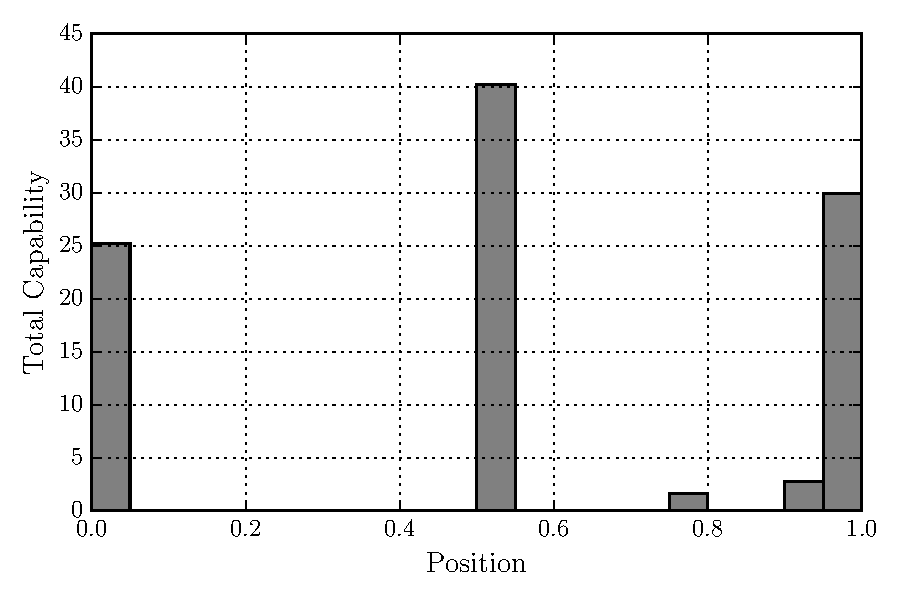
\includegraphics[scale=0.75]{ColdWar/Figures/Original_Inputs_hist}
  \caption[Original Inputs]{Original Inputs -- Initial Distribution of Capabilities}
  \label{fig:original_input_hist}
  \figSpace
 \end{figure}

%% [WGK]: 2. I’m concerned about what the numbers mean and with the lack of consistency in the use of significant figures in tables means for the content. Table 2.1, is mostly 3 significant figures. Ok, but they don’t seem to be when 13 of the 36 values for the position are the same, to 3 significant figures (0.507), yet there another 10 within 0.015. A histogram would be interesting and raise or dispel questions about the workings of the model. Related, Table 2.3, has numbers with apparently 2, 3, and 5 significant figures. How to they interact and what would the histogram tell us?


I then attempt to reproduce the input data from the current, up-to-date COW datasets \citep{gibler_2009,grieg_2010}; however, this did not result in the same inputs as provided in \citet{bdm_1998}. The initial difference is the capability scores -- not just the Composite Index of National Capability (CINC) scores themselves of the various countries for 1948, but their rankings as well. This is likely due to updated data and methodologies, but already indicates a difficulty in replicating the previous study. Since in this case I have access to all the countries for which there is 1948 data, I will include all of them in the model, rather than utilize an arbitrary cutoff.

Next, we must assign each agent to a position. To do so, I construct an undirected network from the most recent COW alliance data for 1948, where the edge between each pair of countries is coded based on the alliance type, as summarized in Table \ref{table:alliance_types}. We can then calculate similarity scores between the the actors' rows or columns in the adjacency matrix, which represent the actors' alliance portfolio. To maintain correspondence with the previous data, I use the tau-b similarity score between portfolios. 

\begin{table}[!h]
\centering
  \caption[Alliance Coding]{Alliance Coding \citep[descriptions quoted from][]{gibler_2013}}
  \label{table:alliance_types}
\begin{tabular}{p{2cm}p{6cm}}
\hline
Alliance Code & Type  \\
\hline
1             & Entente: ``one or both states in the dyad had an understanding that consultations with the other state in the dyad would take place if a crisis occurred.'' \\
2             & Non-Aggression: ``one or both states in the dyad had a non-aggression pact with the other state in the dyad.'' \\
3             & Neutrality: ``one or both states in the dyad had a neutrality pact with the other state in the dyad.'' \\
4             & Defense: ``one or both states in the dyad had a defense pact with the other state in the dyad.'' \\
\hline                                               
\end{tabular}
  \tableSpace
\end{table}

\begin{figure}[!h]
  \centering
  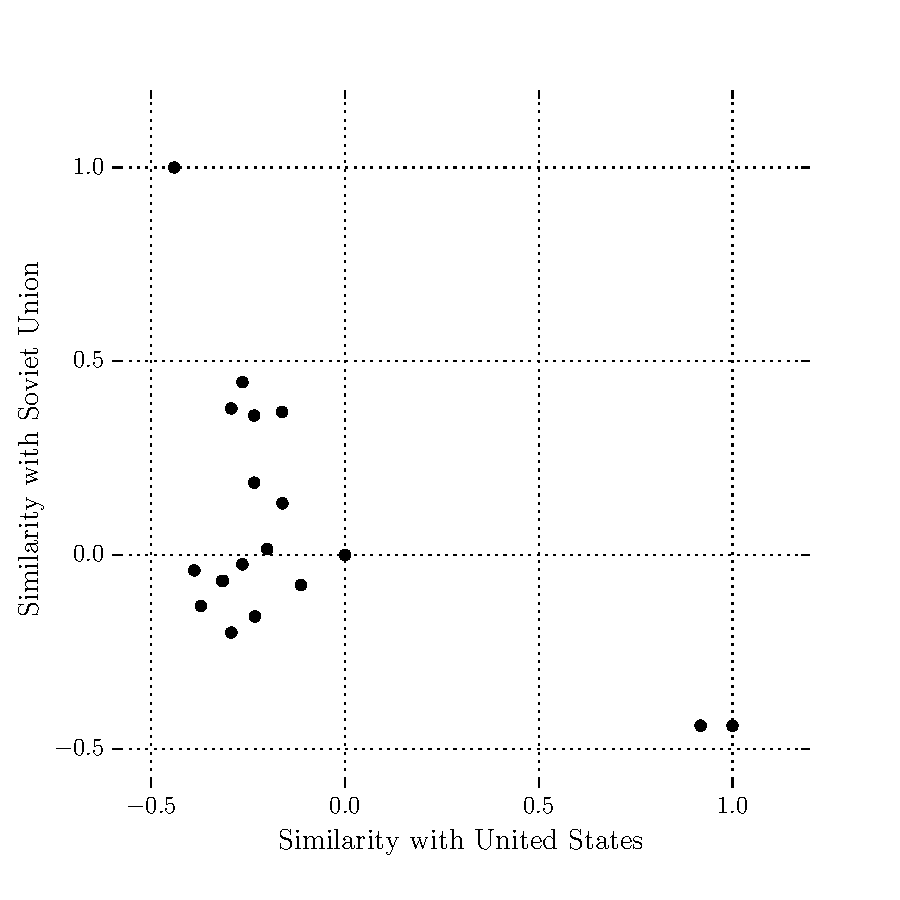
\includegraphics[scale=0.5]{ColdWar/Figures/us_sov_similarities}
  \caption{Tau-b Similarities of Actors to United States and Soviet Union}
  \label{fig:us_sov_corr}
  \figSpace
 \end{figure}

It is here that we run into a question unaddressed in \citet{bdm_1998}. Comparing each country's alliance portfolio to those of the United States and the Soviet Union produces not a single value per country, but two: one for each superpower. As shown in Figure \ref{fig:us_sov_corr}, the relationship between the similarities is not completely linear, meaning we need to choose a way to reduce the two-dimensional security position space to one dimension. Since the two dimensions are highly correlated (correlation coefficient $-0.81$), I use principal component analysis \citep{tipping_1999} to project the two-dimensional data onto a one-dimensional space, which I then rescale so that the values are between 0 and 1.

I term the new model inputs, appropriately enough, the Updated Input data; Table \ref{table:new_inputs} reports the new positions and capabilities\footnote{To make this data directly comparable with the Original Inputs in Table \ref{table:bdm_inputs}, I have rescaled the CINC scores so that they sum to 100. Since Capability scores are used solely as ratios, this rescaling has no effect on the model.}. This input set includes all the countries for which data is available in 1948. Like the Original Input data, it excludes Japan and West and East Germany, which had not yet become sovereign at that point. 
Figure \ref{fig:updated_input_hist} visually shows the initial distribution of power in this scenario: while in this case the United States and its core allies have an even larger advantage over the Soviet Union and its core allies than in the Original Input. The key difference, however, is that instead of a single bloc between the two powers' positions, there are agents at multiple intermediate positions; the single largest power bloc at approximately 0.6, dominated by China and India, is slightly closer to the United States, but there are more agents whose positions are closer to that of the Soviet Union.

\begin{figure}[h!]
  \centering
  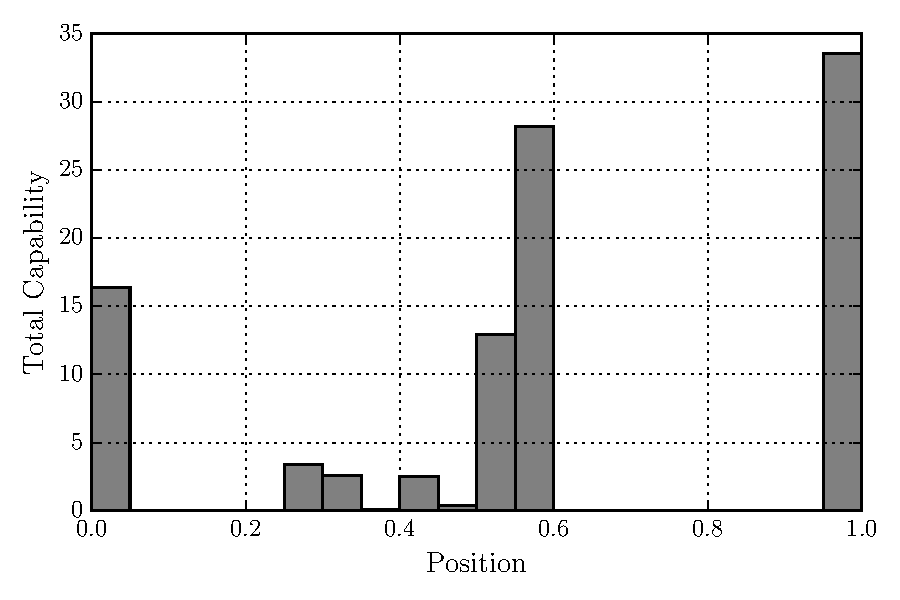
\includegraphics[scale=0.75]{ColdWar/Figures/Updated_Inputs_hist}
  \caption[Updated Inputs]{Updated Inputs - Initial Distribution of Capabilities}
  \label{fig:updated_input_hist}
  \figSpace
 \end{figure}

\begin{landscape}
\begin{table}
  \centering
  \caption{Updated Inputs}
  \label{table:new_inputs}
  \begin{tabular}{lcc||lcc||lcc}
  \hline
  Country            & Capability & Position & Country     & Capability & Position & Country                  & Capability & Position \\
  \hline
Afghanistan        & 0.23       & 0.58     & Haiti       & 0.04       & 0.98     & Paraguay                 & 0.04       & 0.98     \\
Albania            & 0.09       & 0.36     & Honduras    & 0.02       & 0.98     & Peru                     & 0.17       & 0.98     \\
Argentina          & 0.82       & 0.98     & Hungary     & 0.41       & 0.30     & Philippines              & 0.33       & 0.56     \\
Australia          & 0.83       & 0.57     & Iceland     & 0.00       & 0.56     & Poland                   & 2.98       & 0.30     \\
Belgium            & 1.09       & 0.42     & India       & 5.23       & 0.56     & Portugal                 & 0.26       & 0.46     \\
Bolivia            & 0.06       & 0.98     & Iran        & 0.43       & 0.51     & Romania                  & 0.55       & 0.34     \\
Brazil             & 1.22       & 0.98     & Iraq        & 0.13       & 0.49     & Russia                   & 16.36      & 0.00     \\
Bulgaria           & 0.31       & 0.42     & Ireland     & 0.10       & 0.56     & Saudi Arabia             & 0.11       & 0.59     \\
Canada             & 1.26       & 0.56     & Israel      & 0.14       & 0.56     & South Africa             & 0.52       & 0.56     \\
Chile              & 0.20       & 0.98     & Italy       & 1.92       & 0.56     & Spain                    & 1.48       & 0.57     \\
China              & 11.48      & 0.57     & Jordan      & 0.02       & 0.52     & Sri Lanka                & 0.09       & 0.56     \\
Colombia           & 0.26       & 0.98     & Lebanon     & 0.03       & 0.59     & Sweden                   & 0.60       & 0.56     \\
Costa Rica         & 0.01       & 0.98     & Liberia     & 0.01       & 0.56     & Switzerland              & 0.20       & 0.56     \\
Cuba               & 0.17       & 0.98     & Luxembourg  & 0.29       & 0.42     & Syria                    & 0.09       & 0.59     \\
Czechoslovakia     & 1.26       & 0.34     & Mexico      & 0.66       & 0.98     & Thailand                 & 0.34       & 0.56     \\
Denmark            & 0.21       & 0.56     & Mongolia    & 0.04       & 0.57     & Turkey                   & 1.17       & 0.51     \\
Dominican Republic & 0.06       & 0.98     & Myanmar     & 0.23       & 0.56     & United Kingdom           & 7.52       & 0.54     \\
Ecuador            & 0.09       & 0.98     & Nepal       & 0.11       & 0.56     & United States of America & 29.39      & 1.00     \\
Egypt              & 0.54       & 0.52     & Netherlands & 0.83       & 0.42     & Uruguay                  & 0.08       & 0.98     \\
El Salvador        & 0.03       & 0.98     & New Zealand & 0.09       & 0.57     & Venezuela                & 0.13       & 0.98     \\
Ethiopia           & 0.23       & 0.56     & Nicaragua   & 0.01       & 0.98     & Yemen Arab Republic      & 0.06       & 0.59     \\
Finland            & 0.19       & 0.57     & North Korea & 0.36       & 0.56     & Yugoslavia               & 0.80       & 0.32     \\
France             & 3.25       & 0.51     & Norway      & 0.16       & 0.56     &                          &            &          \\
Greece             & 0.36       & 0.56     & Pakistan    & 1.18       & 0.56     &                          &            &          \\
Guatemala          & 0.07       & 0.98     & Panama      & 0.01       & 0.98     &                          &            &   \\      
  \hline
\end{tabular}

  \tableSpace
\end{table}
\end{landscape}

%% [WGK]: 2. ... Related, Table 2.3, has numbers with apparently 2, 3, and 5 significant figures. How to they interact and what would the histogram tell us?
  % --> DONE

\subsection{Model Instantiations} \label{models}

I use the input datasets above to instantiate two model variants, drawn from the previous chapter's Section 3.7.3. The first corresponds to Model 1a, and is the attempt to reproduce the EUM as originally described across multiple papers \citep{bdm_1994,bdm_1997,bdm_2002}; I will refer to this as the Baseline model. The second corresponds to Model 2b, chosen because it was the most predictive of the ICEWS events in the previous chapter; I will refer to this as the Updated model.

These model variants differ from the versions in the previous chapter in their salience updating sub-model. As \citet{bdm_1998} notes, there are countless unpredictable elements affecting how states will perceive, and act on, their international security interests in the context of the Cold War, from domestic political changes to natural disasters. Rather than extend the model to explicitly capture more and more of these factors, we implicitly incorporate them by randomizing agent salience values. At the beginning of each step of the model, each agent's salience is randomly drawn from a uniform distribution over the ${[0, 1]}$ range -- this is salience sub-model variant $\mathbf{S_{1,1}}$, in the notation presented in the previous chapter. Since capability is always multiplied by salience, this effectively adds a noise factor to the agents' strength as well. While agents with greater capabilities are likely to remain stronger than ones with lower capabilities, there exist configurations of salience values under which the generally weaker agent temporarily has an advantage over a stronger agent.

% RAX: Can [the previous paragraph] be justified in any way? 
% Not that I know of? 

In the notation introduced in the previous chapter, these models can be denoted as:

\begin{description}
  \item[Baseline:] $\{\mathbf{T_0, S_{1,1}, W_0, R_0, O_0, M_0, A_0}\}$ 
  \item[Updated:] $\{\mathbf{T_1, S_{1,1}, W_1, R_1, O_0, M_1, A_0}\}$
\end{description}

Taken together, the two model variants and two input datasets yield four experiments in all, as shown in Table \ref{table:experiment_matrix}.

\begin{table}
  \centering
  \caption{Experiment Summary}
    \label{table:experiment_matrix}
  \begin{tabular}{l|cc}
  \hline
                & Baseline Model &  Updated Model \\
  \hline
  Original Inputs & Experiment 1   & Experiment 2   \\
  Updated Inputs  & Experiment 3    & Experiment 4  \\
  \hline
\end{tabular}
    \tableSpace
\end{table}

For all experiments, I instantiate all agents with parameters $Q=0.5$ and $T=0.5$ indicating maximum uncertainty about the world. Each model is run for 25 steps. \citet{bdm_1998} hypothesizes that this is roughly equivalent to 50 years of history, meaning that agents experience salience shocks, engage in conflicts, and change position approximately once every two years. With 1948 as the starting year, the models will generate data corresponding approximately to 1998 as the end year.

To briefly restate the model: during each step, each agent evaluates its expected utility from threatening conflict against each other agents in an attempt to coerce the other agents to adopt its current position; when that expected utility is positive, the agent issues the threat. The agents then evaluate all their incoming threats, choosing the one requiring the least movement, and moving based on their own expected utility (interpreted here as fear of a conflict), either compromising and moving slightly towards the threat sender's position or capitulating and adopting that position outright. In the Baseline variant, but not the Updated one, if agent A chooses B's threat, while B chooses C's threat, B backs out of its decision and does not move. 

If two agents threaten each other and do not choose to compromise with or capitulate to another agent, they enter into a conflict. All agents then contribute capability to the side they prefer, in proportion with the strength of their preference. The winner is chosen randomly, with probabilities based on each agent's share of total capability contributed to the conflict. In the Baseline variant, the loser of a conflict adopts the winner's position; in the Updated variant, neither agent changes position, regardless of the conflict outcome.

Due to the large number of independent random variables driving the model, I run 1,000 instantiations of each experiment. This number appears to be  sufficiently large to sample from the many different possible configurations of saliences and conflict outcomes\footnote{excursions using 10,000 instantiations did not produce meaningfully different outcome distributions.}. Furthermore, since we are concerned with commonly-emerging outcomes and behaviors, particular phenomena occurring less frequently than in 0.1\% of model runs are unlikely to be of practical interest.

%% [WGK] 1. Between the inputs and outputs, I suggest a little review of the processing of the model and possibly whether each round, representing ~2yrs, includes all agents making offers, etc. Related, are there any in process indicators other than the resulting overall positions, such as a track of an individual country’s relationship with the US and USSR? Jumping from inputs to outputs with no discussion of the process in between is uncomfortable.
  % --> DONE!


\subsection{Output Data} \label{outputs}

Each model run generates several outputs. At the beginning of each step of the run, it records the position currently held by each agent, as well as the current median voter position, and capability-weighted mean position. During each step, the model also logs all conflicts which occur between agents. I collect and aggregate these outputs across all 1,000 runs of each experiment.

I then compare these outputs to two Correlates of War datasets: militarized interstate disputes (MIDs) for the 1948-1998 timeframe, and alliance data for 1998. The MID dataset provides an expert-coded listing of all cases where one state threatened or used force against another \citep{jones_1996}. While there are many forms of conflict, militarized disputes, which can escalate into wars, are particularly important to the international system, and thus of particular interest for forecasting. I will attempt to see whether the number of conflict events between pairs of actors generated by the model runs is a useful predictor of the number of conflicts between states in the relevant time period. 

Similarly, the model runs produce traces of agent positions. Agents with closer positions are more likely to support one another more strongly in conflict with other agents, i.e. they behave the way we would expect allied countries to behave. Thus, I will test whether the distance between agents is a predictor of alliances between the corresponding countries.

\section{Results} \label{results}

\subsection{Overview}

The initial question posed by \citet{bdm_1998} was whether the end of the Cold War -- that is, a substantial shift in the median international security position to the advantage of the United States -- could be generated from the model. Figure \ref{fig:original_cdf} shows the cumulative distribution of model end positions reported by that paper. Note the sharp increase in the cumulative distribution curve very close to 0 (equivalent to 0.5, in the variant used here), indicating that one of the most common types of outcomes is one where the Cold War persists at the end of the model run, with a median position between the starting position of both superpowers and no clear advantage to either side. However, the distribution is also clearly non-symmetric, with more outcomes favoring the United States (closer to +100) than the USSR. The conclusion of the original paper was thus that the end of the Cold War, with an American victory, was not as unforeseeable as others had argued, and in fact could be emerged from the model.

\begin{figure}[h!]
  \centering
  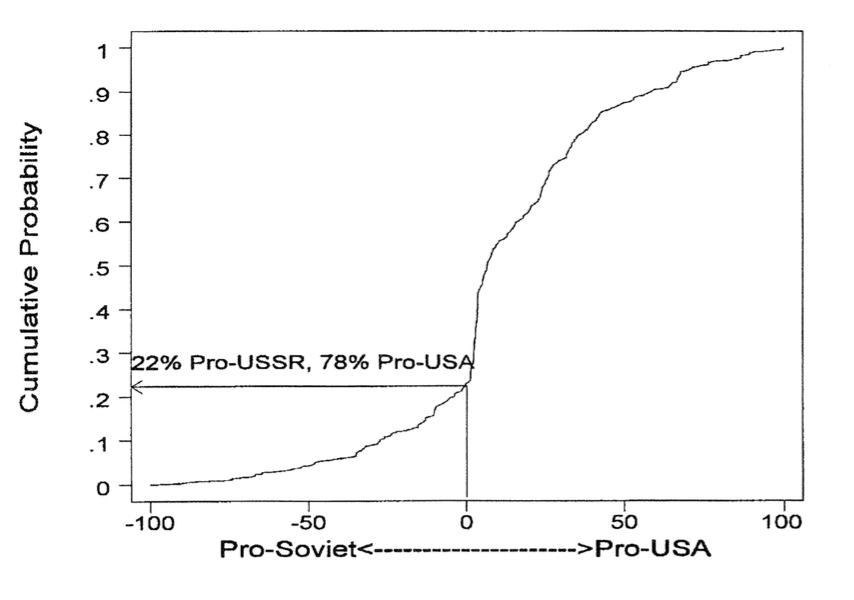
\includegraphics[scale=0.75]{ColdWar/Figures/ColdWarOriginal}
  \caption[Original Model Cumulative Distribution]{Model Outcome Cumulative Distribution, Copied From \citet{bdm_1998} }
  \label{fig:original_cdf}
  \figSpace
 \end{figure}

Figure \ref{fig:new_cdfs} shows the same cumulative distributions across the four experiments\footnote{\citet{bdm_1998} does not provide all the results of each model run, meaning that we cannot directly superimpose the results shown in Figures \ref{fig:original_cdf} and \ref{fig:new_cdfs}.}. Immediately, we note that the overall shapes are similar, though not identical. The bulk of outcomes are very close to the center, with substantially more US-victory outcomes than USSR-victory ones. In particular, Experiment 1, which attempts to replicate the original model, has almost no USSR-victory outcomes, and more outcomes where the median position does not indicate a victory to either side.

\begin{figure}[h!]
  \centering
  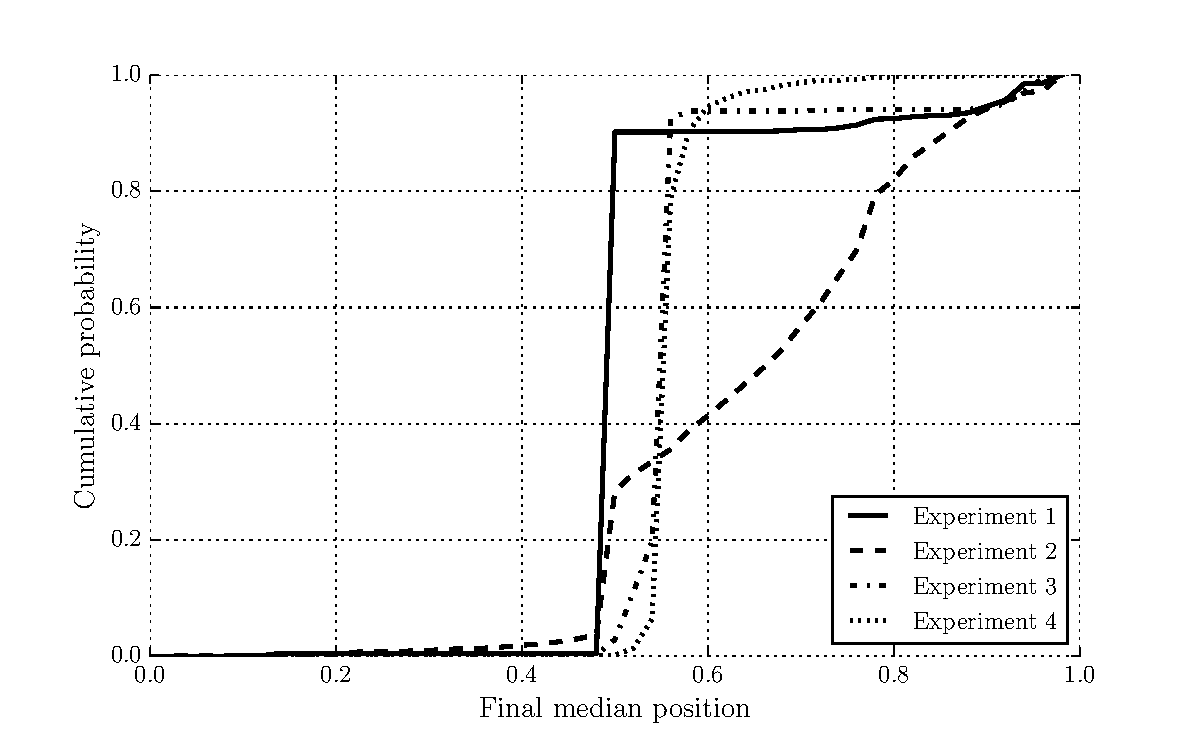
\includegraphics[scale=0.5]{ColdWar/Figures/Model_cdfs}
  \caption[New Model Cumulative Distribution]{Model Outcomes Cumulative Distributions}
  \label{fig:new_cdfs}
  \figSpace
 \end{figure}


%% [WGK] 3. Can Figure 2.3 (or an additional figure prior to 2.3) show us the range of values from all the runs rather than just the mean? Either standard error bands or all the runs plotted on top of each other?



\begin{figure}[t!]
    \centering
    \begin{subfigure}[t]{0.49\textwidth}
        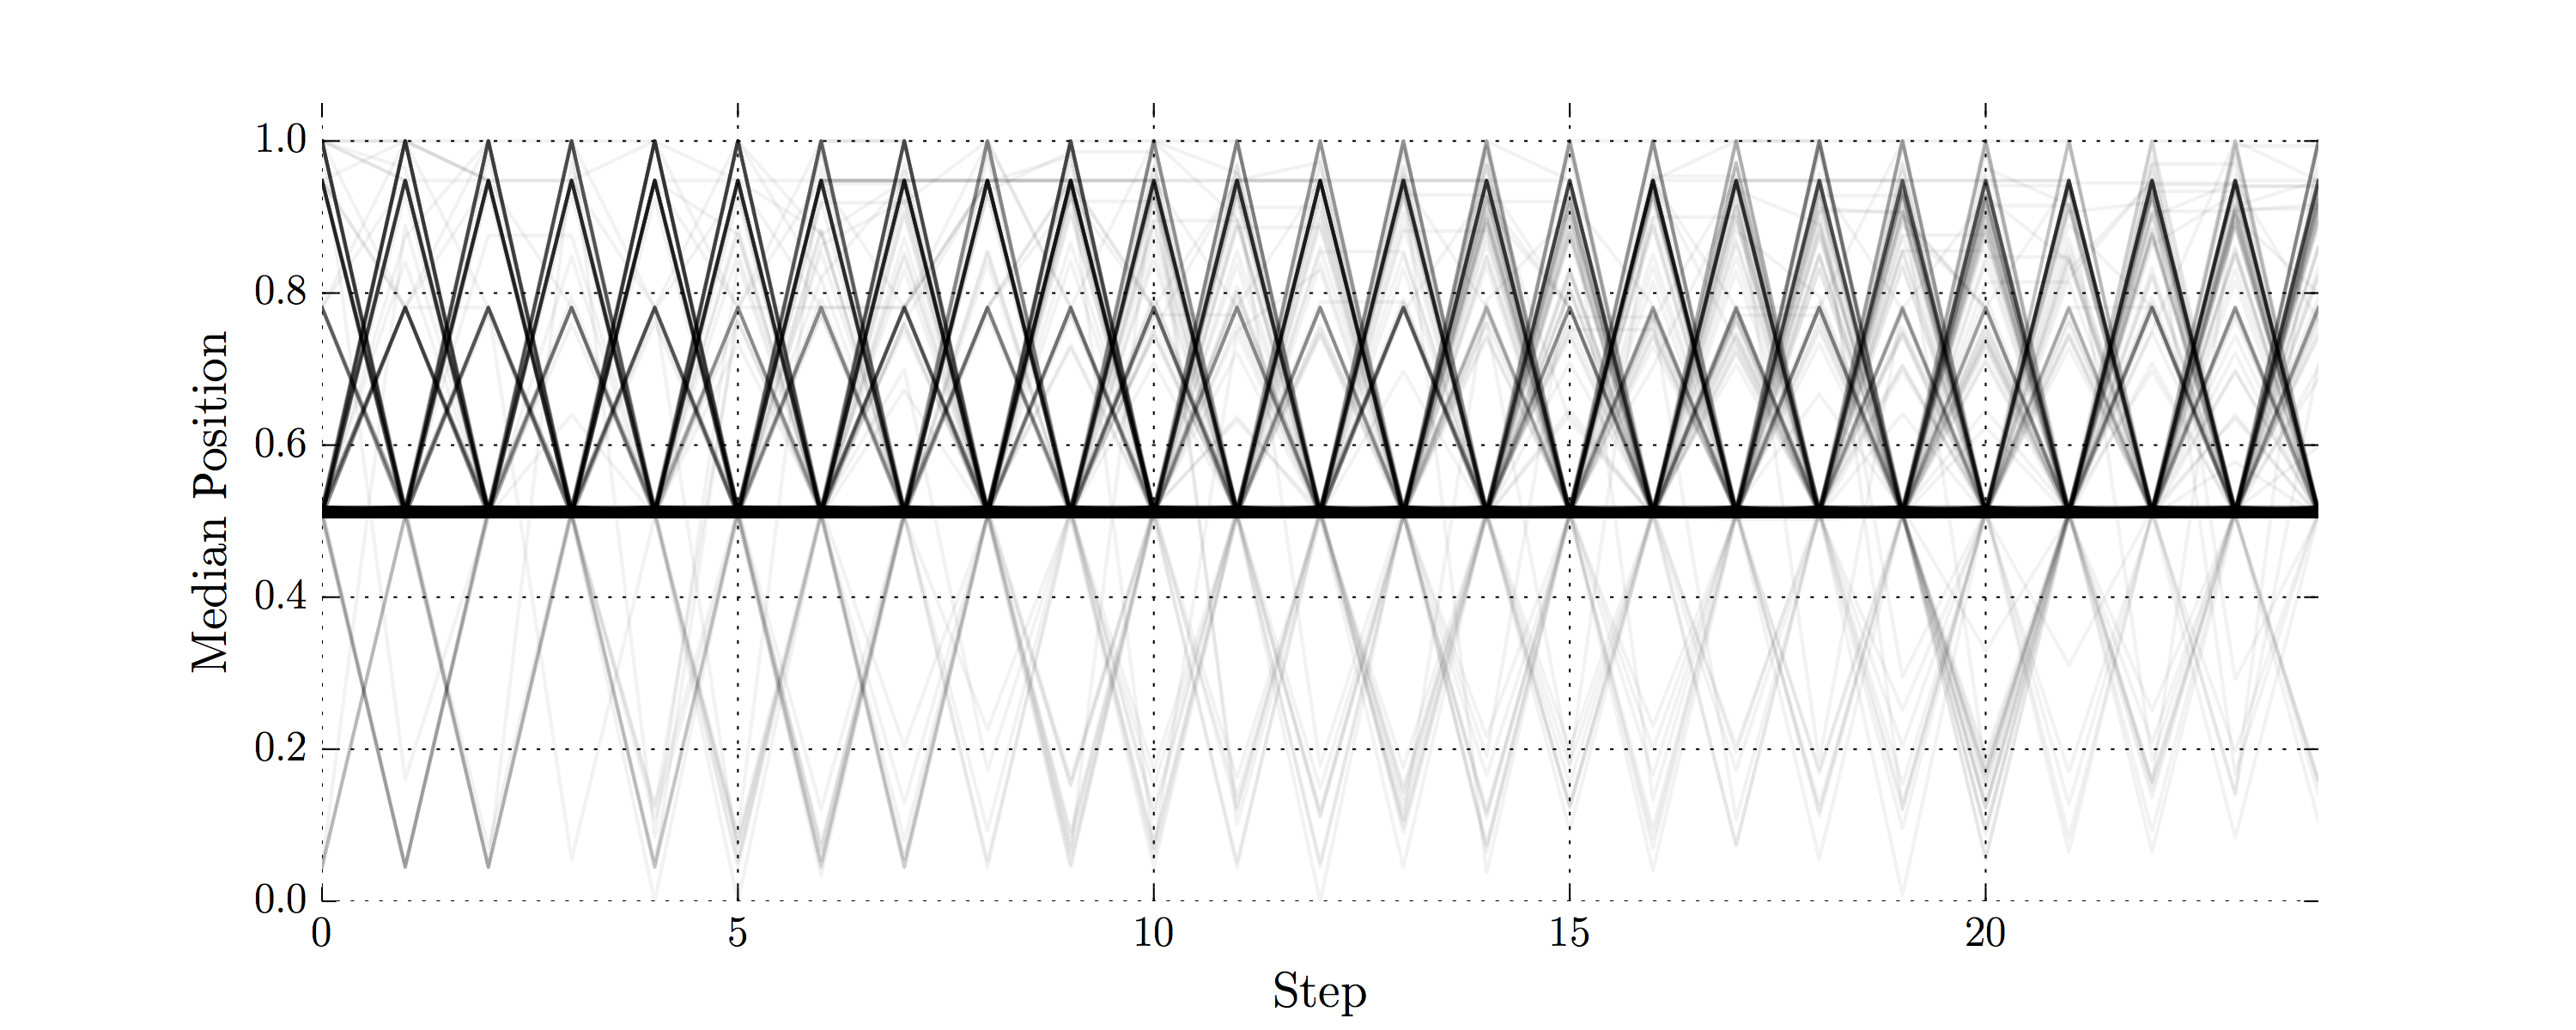
\includegraphics[width=\textwidth]{ColdWar/Figures/Exp1_traces}
        \caption{Experiment 1}
    \end{subfigure}
    \begin{subfigure}[t]{0.49\textwidth}
        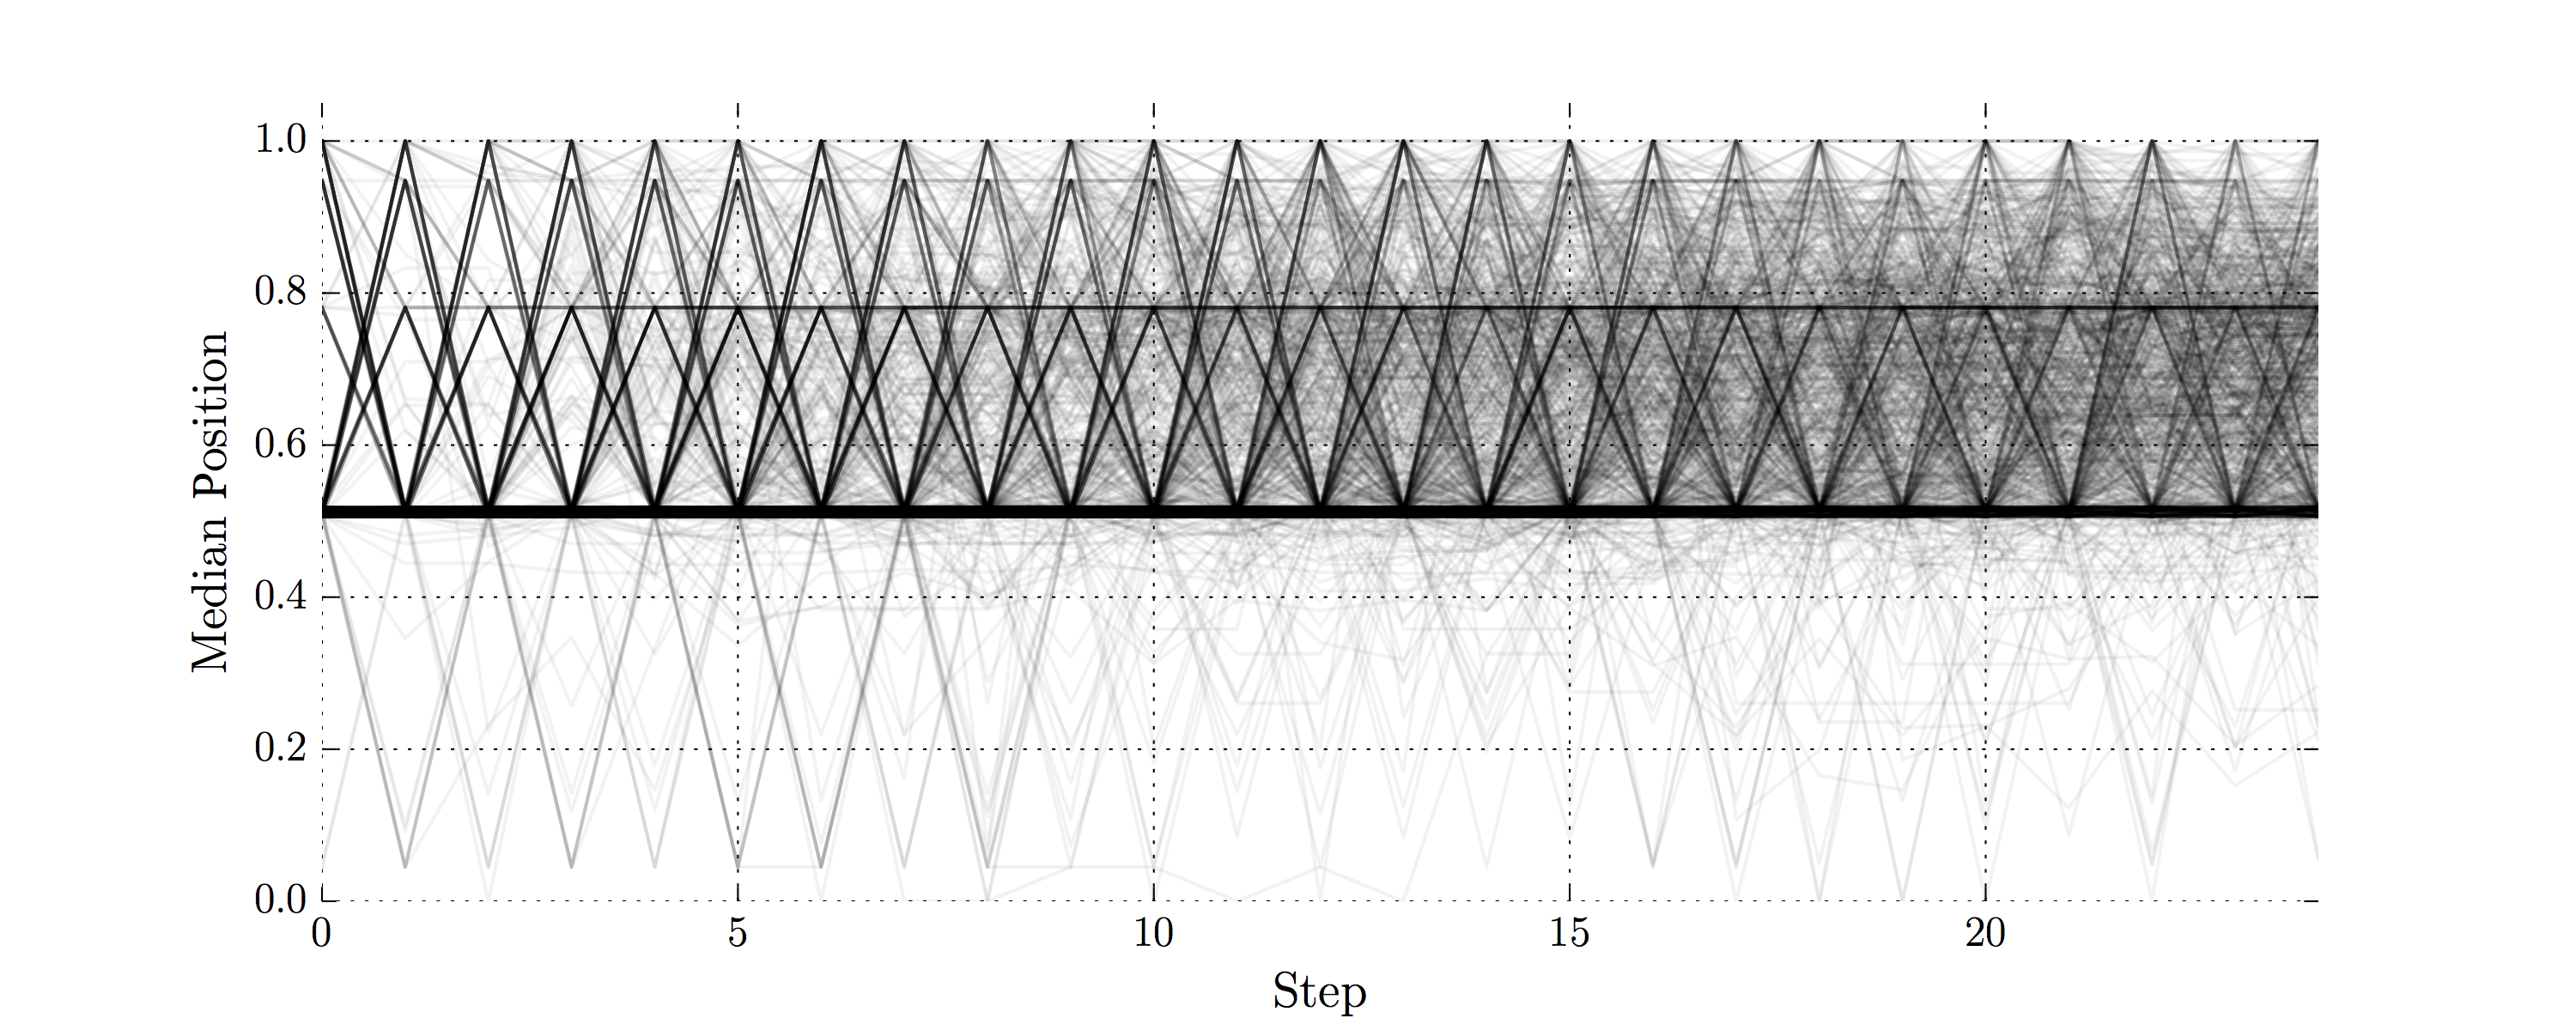
\includegraphics[width=\textwidth]{ColdWar/Figures/Exp2_traces}
        \caption{Experiment 2}
    \end{subfigure}

    \begin{subfigure}[t]{0.49\textwidth}
        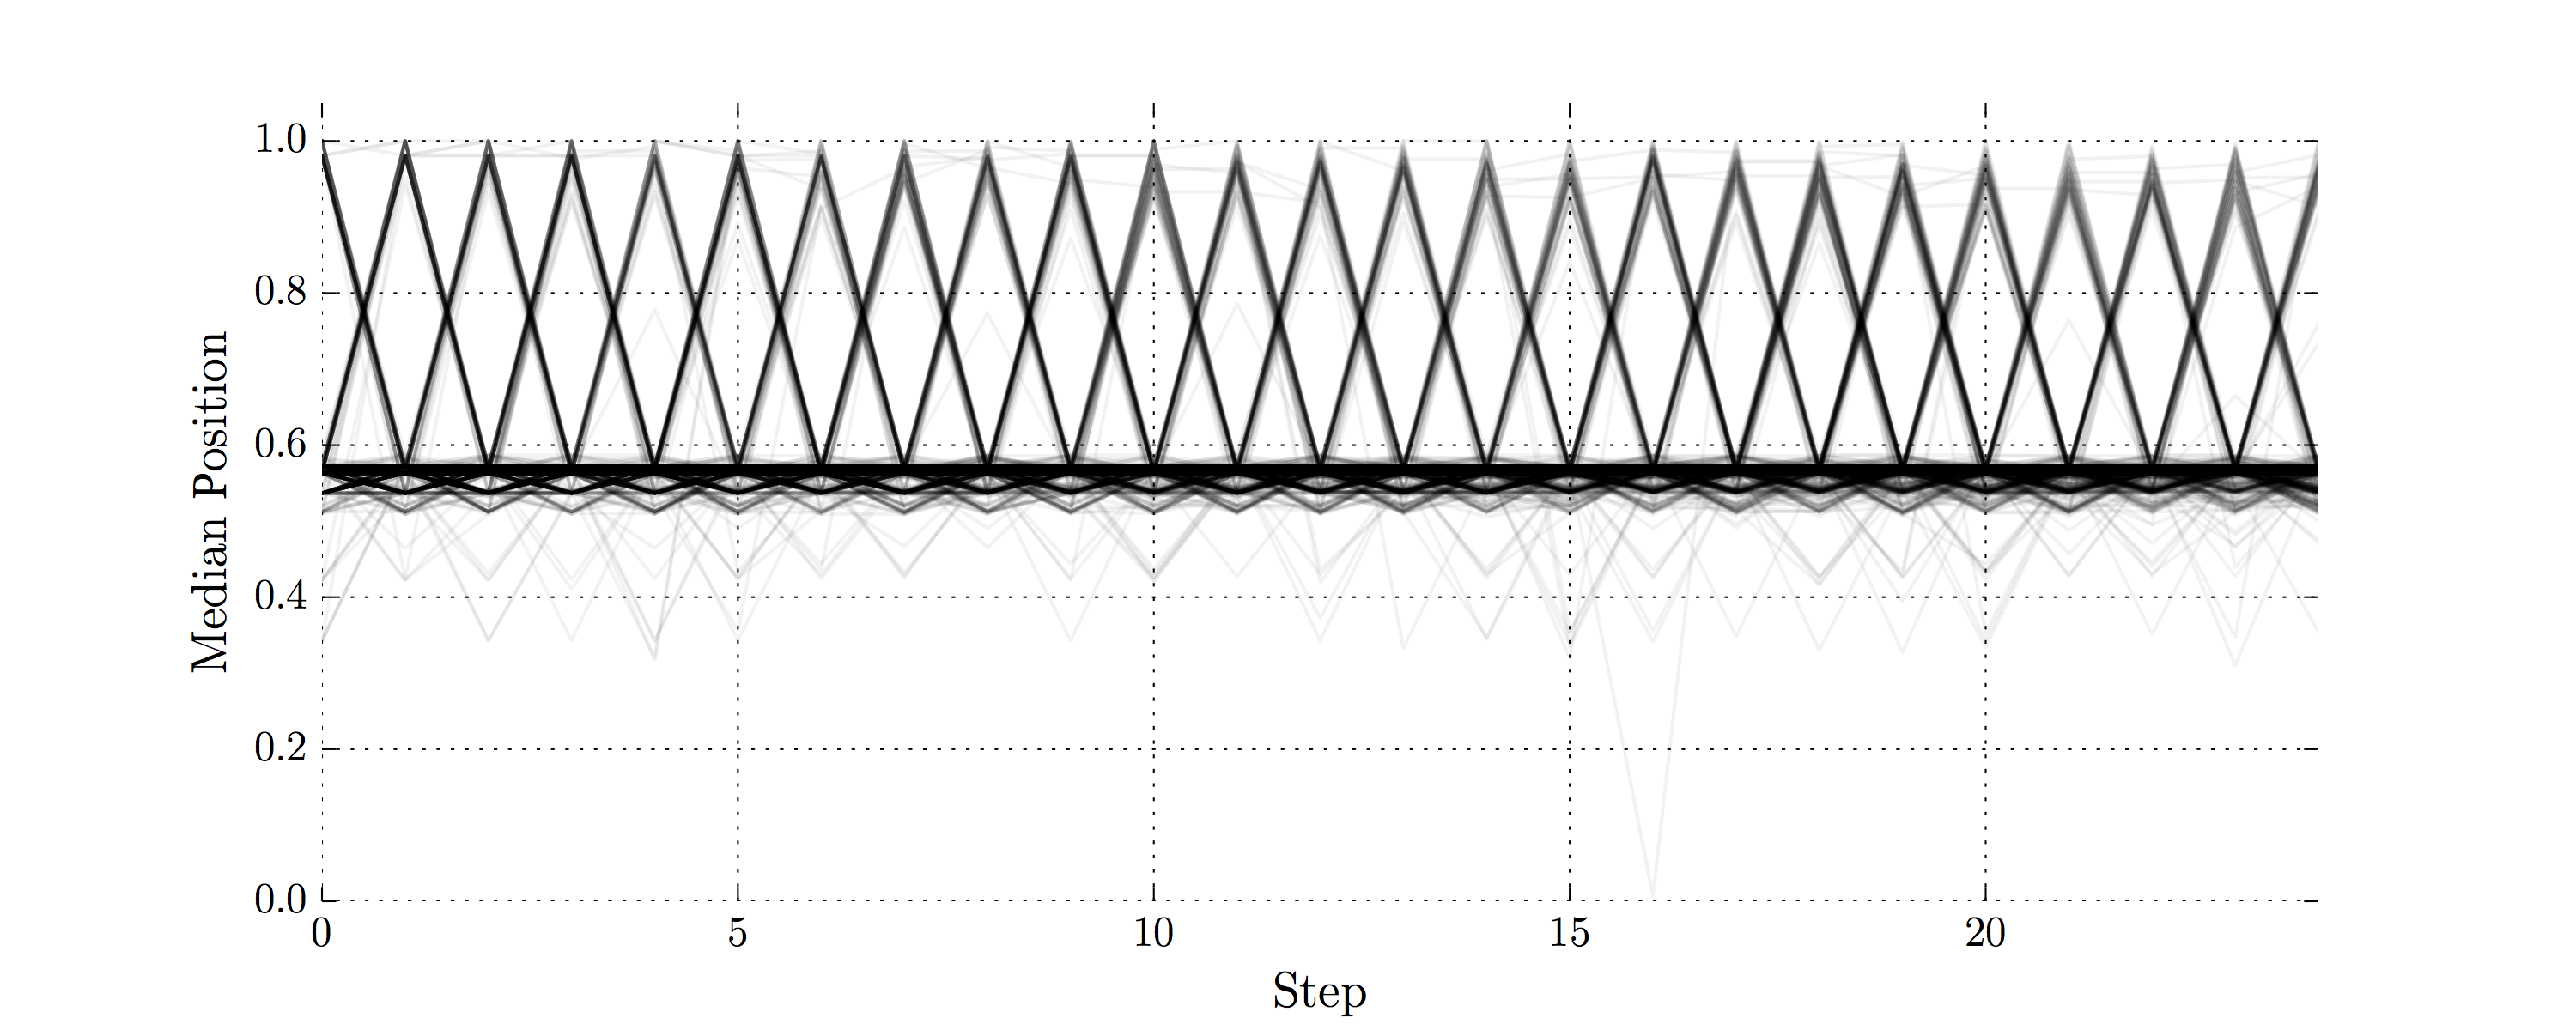
\includegraphics[width=\textwidth]{ColdWar/Figures/Exp3_traces}
        \caption{Experiment 3}
    \end{subfigure}
    \begin{subfigure}[t]{0.49\textwidth}
        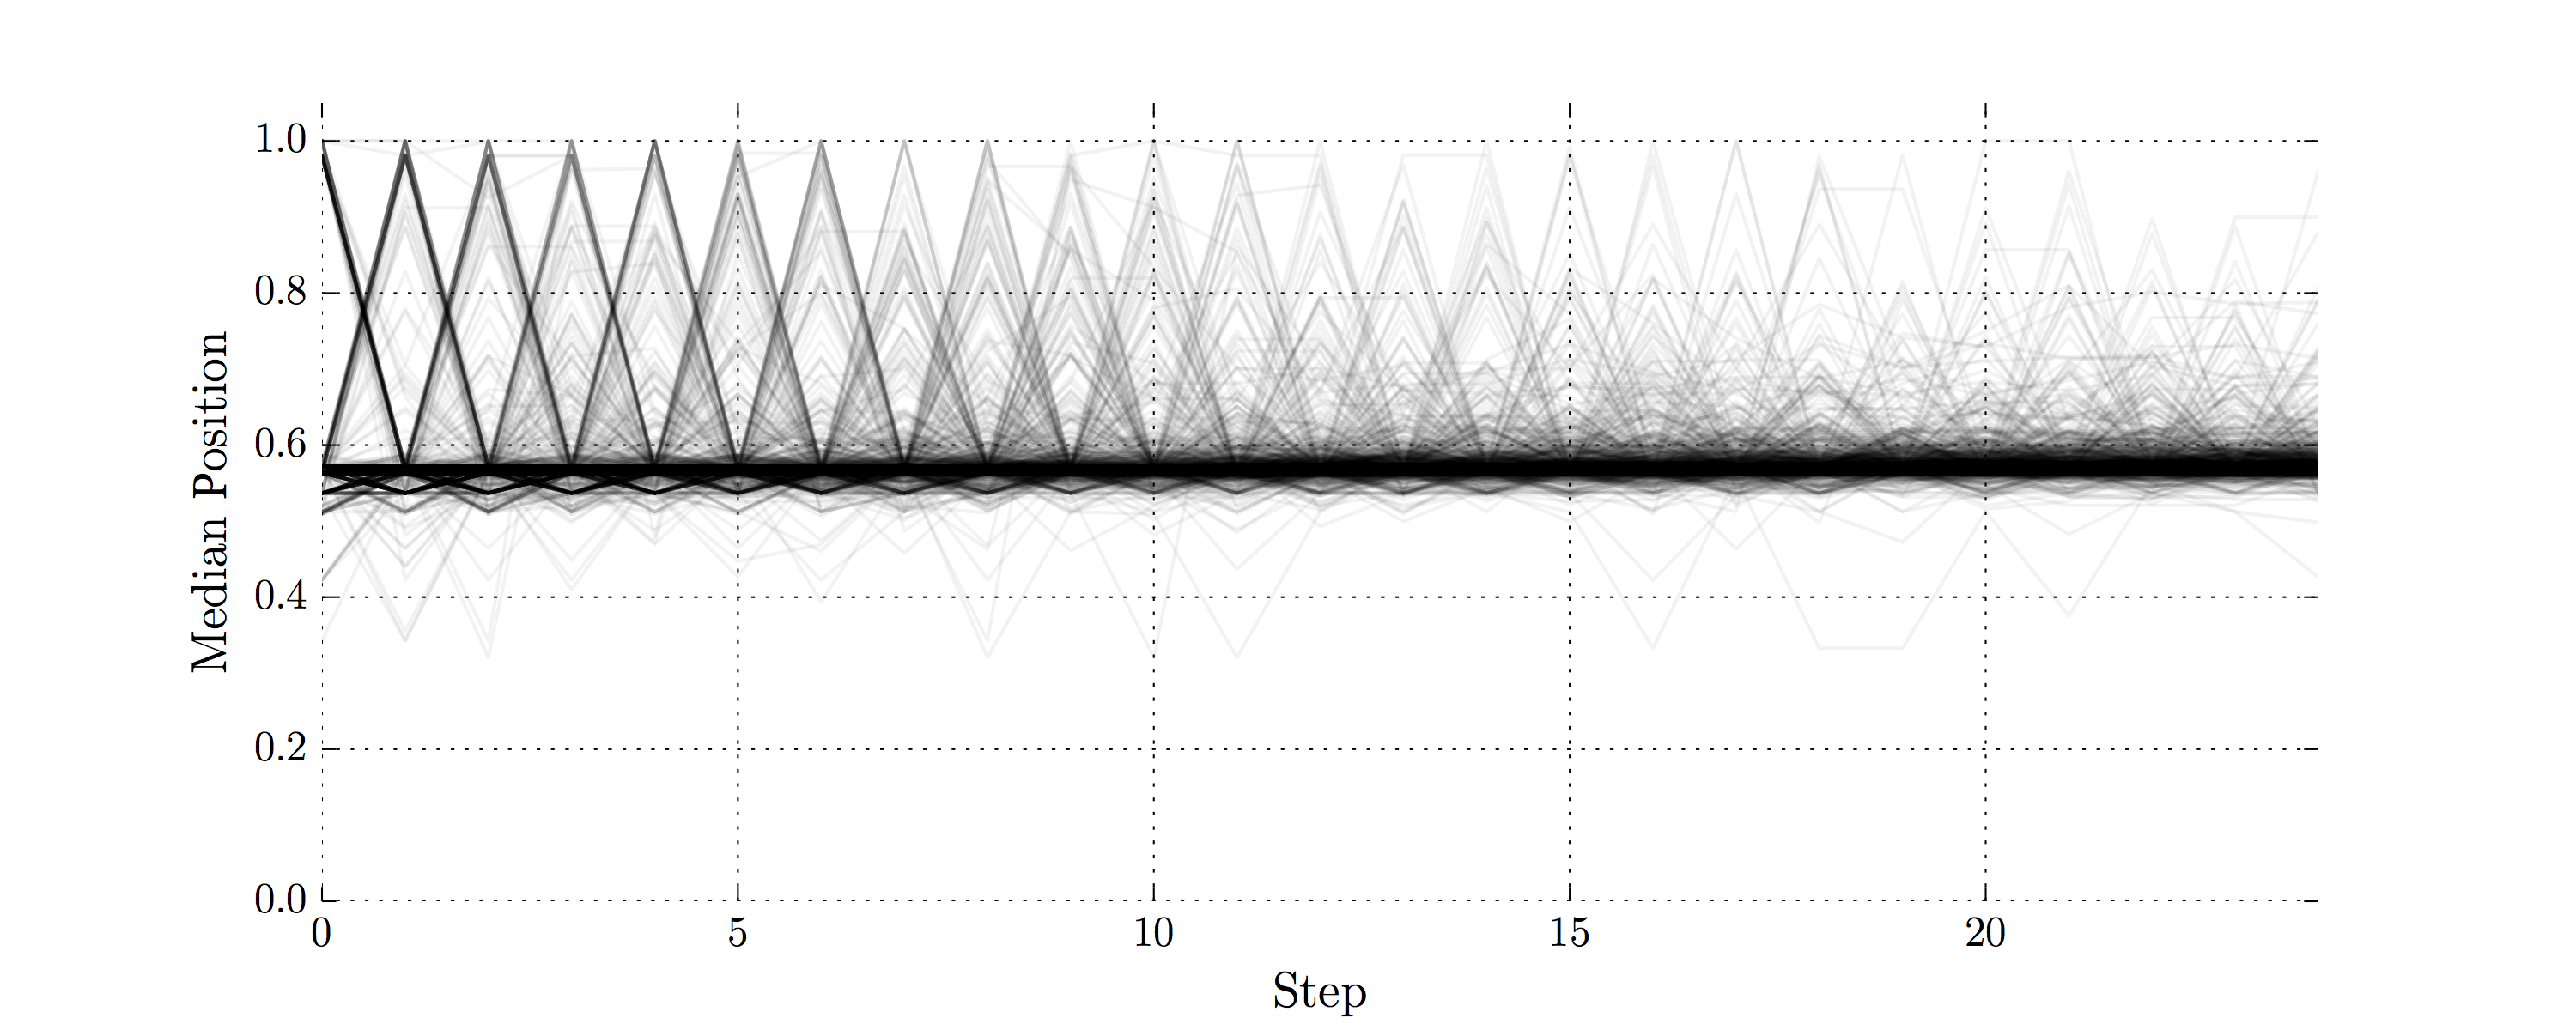
\includegraphics[width=\textwidth]{ColdWar/Figures/Exp4_traces}
        \caption{Experiment 4}
    \end{subfigure}
    
    \caption{Median Position Traces}
    \label{fig:model_traces}
    \figSpace
\end{figure}

%% [WGK] 4. There’s a description of the results as a sawtooth pattern before figures 2.4 are introduced. The reader can’t know where that comes from. <-- Make sure fig:model_traces appears before words 'sawtooth pattern'


Let us take a closer look at the behaviors these models are generating. Figure \ref{fig:model_traces} shows the superimposed traces of the median position for all the model runs of all experiments. The opacity of each trace line is low, so that the darker a line appears, the more traces exhibited that particular transition. While it is impossible to discern individual runs here, these visualizations serve to highlight recurring patterns. Two patterns are obvious across all four experiments. The first is that, as the cumulative distributions in Figure \ref{fig:new_cdfs} suggest, the most common positions for the model at any given step are at or close to the starting median -- by and large, the median does not change very often. The next key pattern is that, across all the experiments, the median position exhibits a sawtooth pattern, diverging from the 0.5 position towards one extreme or the other and immediately returning. In other words, one of the sides (though more frequently the United States) gains a brief advantage, and then the status quo quickly reasserts itself. This sawtooth pattern is particularly distinct and uniform in the Baseline model used in Experiments 1 and 3. Experiment 2, and to a lesser extent Experiment 4, show a wider variety of traces. In particular, close examination of the Experiment 2 traces indicates more cases where changes in median are not one-round spikes, but transitions to a new stable position. Finally, Experiment 4 shows a decline in movement as time advances, suggesting that the agents are sorting themselves into a more stable configuration around the same median.

The sawtooth pattern raises a question: do the model runs ending in a US (or Soviet, for that matter) victory represent a true long-term shift in the status quo, or are they simply cases where a temporary spike towards one side or the other coincides with the final step of the model? In fact, a close examination of the model runs suggests that the latter is exactly what is happening in Experiments 1 and 3. Figure \ref{fig:example_traces} shows example traces from randomly-selected runs which end with a median position of 0.7 or greater, indicating a US victory. In the traces from Experiments 1 and 3, the median position exhibits several short-lived excursions away from the starting position, quickly reverting after each. There is no reason to suppose that the spike preceding the end of the run represents a true change from this pattern. The trace from Experiment 2, in contrast, shows that the median position had gone up prior to the final step of the run, and remained relatively stable at its new position. The Experiment 4 trace also shows the run achieving a new stable position, with smaller spikes away from it, including one coinciding with the terminal step. These patterns recur across the runs in each experiment that are not visualized here, including those not ending in a US victory.

A thorough examination of model runs suggests that the spikes -- including the terminal ones -- are driven less by changes in agent positions than by the changes of agent salience values. Importantly, these changes are not accompanied by a similar change in the weighted mean position -- which is to say, not driven by similar changes in the positions of the agents themselves. Recall that as detailed in the previous chapter, in Section 3.2.2, the median is computed by checking which agent position has the highest probability of defeating all other agent positions in bilateral conflicts; thus, they are affected by the stochastic salience changes. In contrast, the mean position is weighted by (fixed) capabilities, and thus is not directly affected by salience variations.

This phenomenon is illustrated in Figure \ref{fig:example_agent_traces}, showing the individual agent positions over time for the same runs as in Figure \ref{fig:example_traces}. In this figure, each line corresponds to an agent: the $y$ axis indicates each agent's position at each step, shown on the $x$ axis; line widths correspond to the agents' capabilities. The top-most line is always the position of the United States agent and the bottom-most line is the USSR agent. The traces for all the experiments show that the radical, temporary spikes in the median position do not correspond to similar sharp shifts in any agent position. In Experiment 1, the agents exhibit a slight movement towards the center of the position space. Note, however, that the movement by the USSR agent and its allies (at the bottom of the graph) are more substantial than those of the US and its aligned agents at the top. In Experiment 3, however, very little movement occurs at all. In Experiments 2 and 4, in contrast, the agents exhibit sharp, more substantial changes in their positions, which correspond to the changes in the median, highlighting that the median change is not being driven solely here by stochastic changes in salience.

In fact, in the Experiment 2 and 4 traces, we can see a particularly interesting story emerge. Early on, several agents whose positions are closer to the median are drawn closer to the position of the United States; this is followed by several Soviet-aligned agents being drawn `upward' towards the United States's preferred position across multiple steps. The Soviet Union itself lags behind these agents for a number of steps. However, eventually it too is driven to adjust its position upwards, in the Experiment 4 trace even eventually joining the US-aligned cluster. In effect, this model generates a recognizable notional history of the Cold War leading to a US-dominated unipolar world. 

\begin{figure}[!htbp]
    \centering
    \begin{subfigure}[t]{0.49\textwidth}
        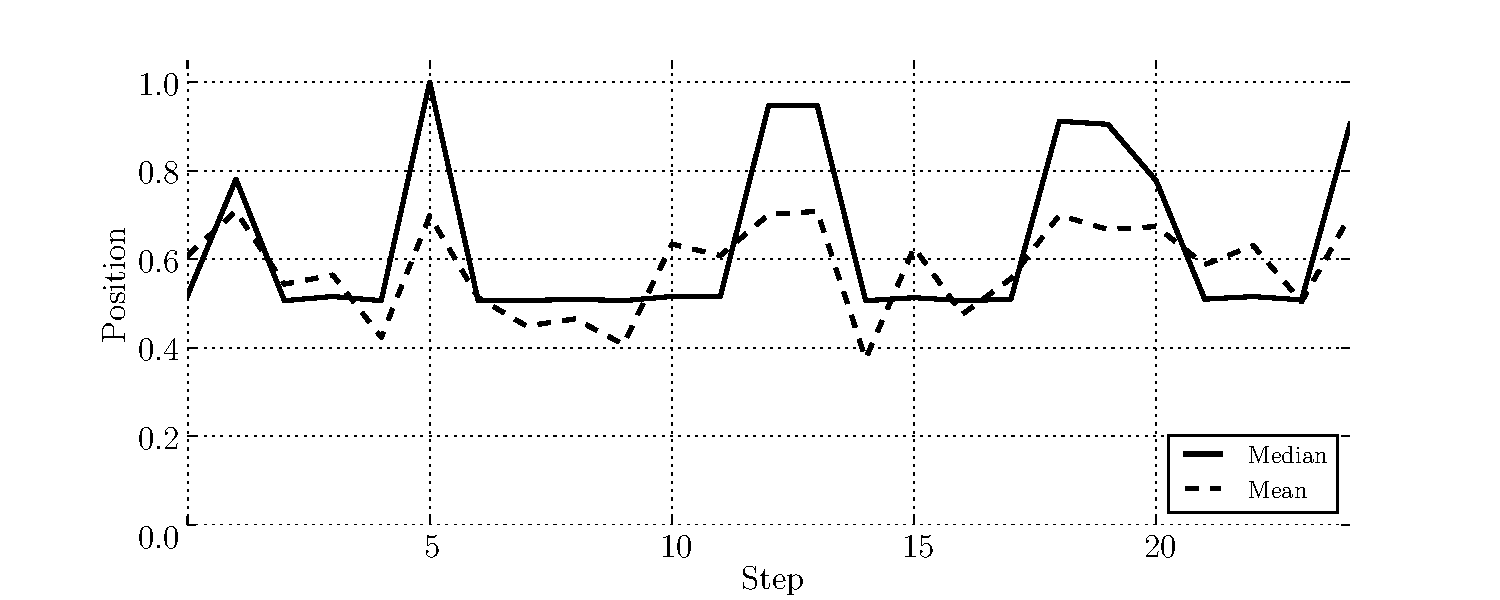
\includegraphics[width=\textwidth]{ColdWar/Figures/Exp1_uswin_trace}
        \caption{Experiment 1}
    \end{subfigure}
    \begin{subfigure}[t]{0.49\textwidth}
        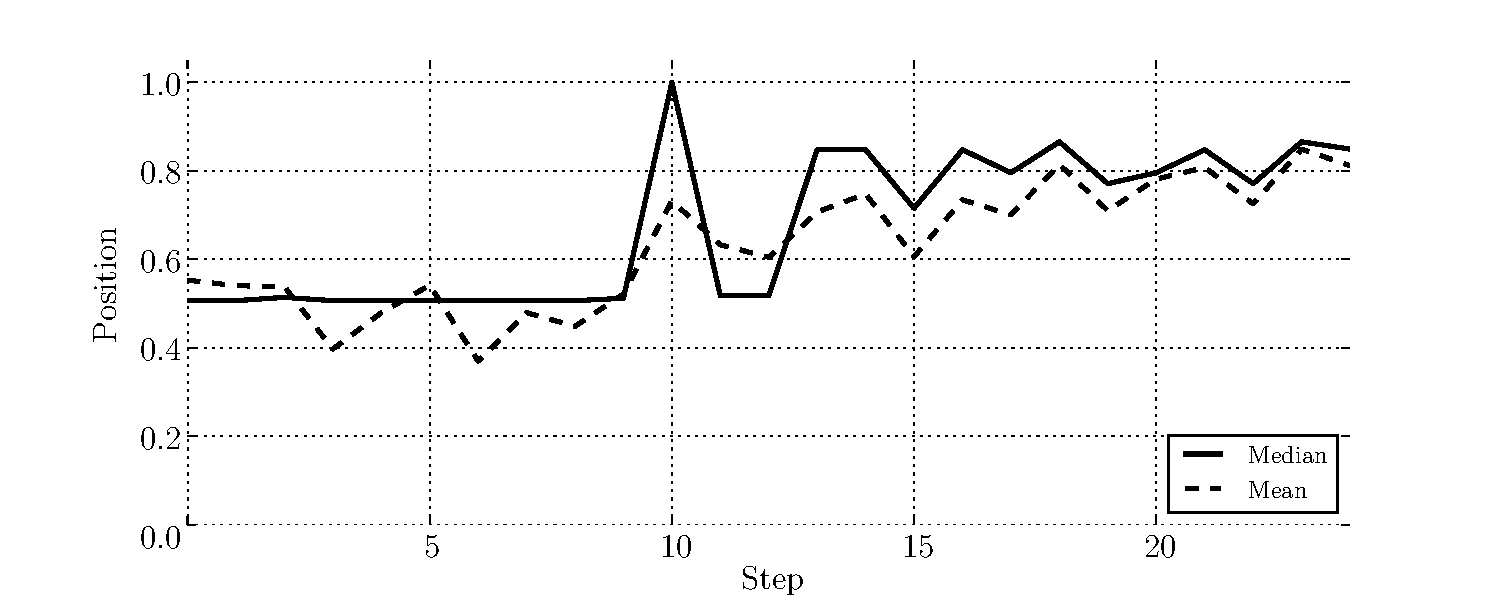
\includegraphics[width=\textwidth]{ColdWar/Figures/Exp2_uswin_trace}
        \caption{Experiment 2}
    \end{subfigure}

    \begin{subfigure}[t]{0.49\textwidth}
        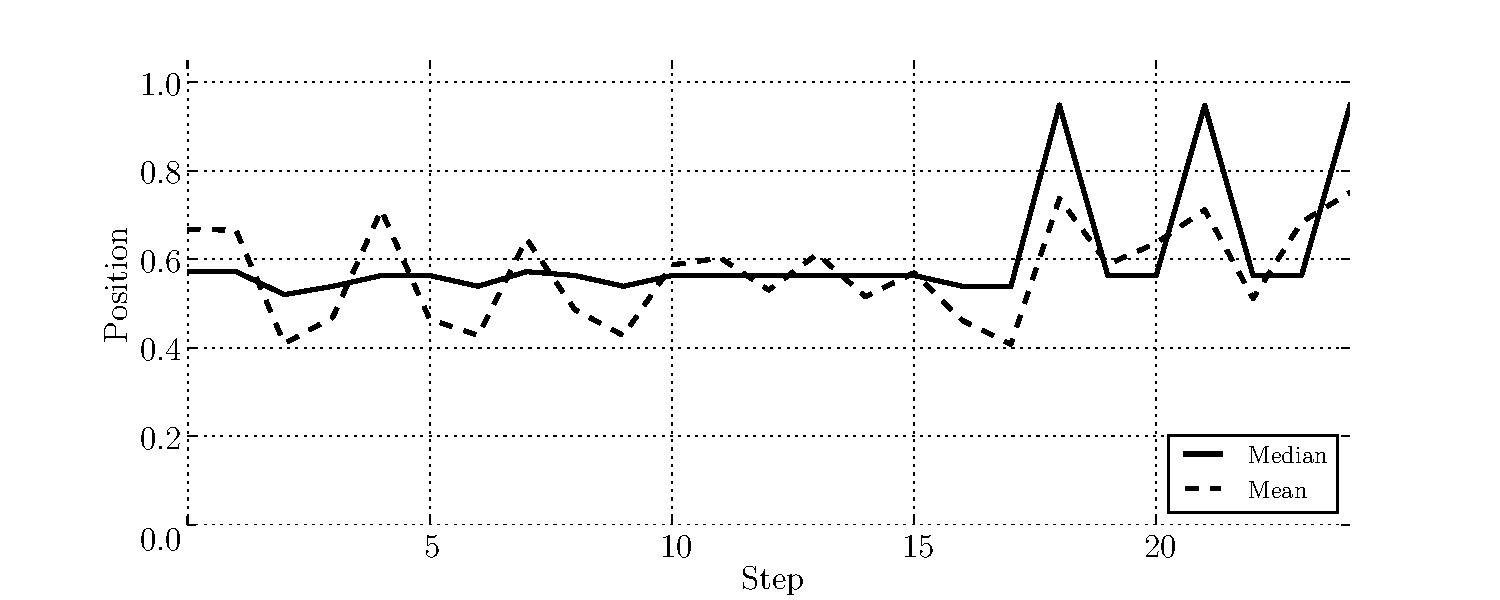
\includegraphics[width=\textwidth]{ColdWar/Figures/Exp3_uswin_trace}
        \caption{Experiment 3}
    \end{subfigure}
    \begin{subfigure}[t]{0.49\textwidth}
        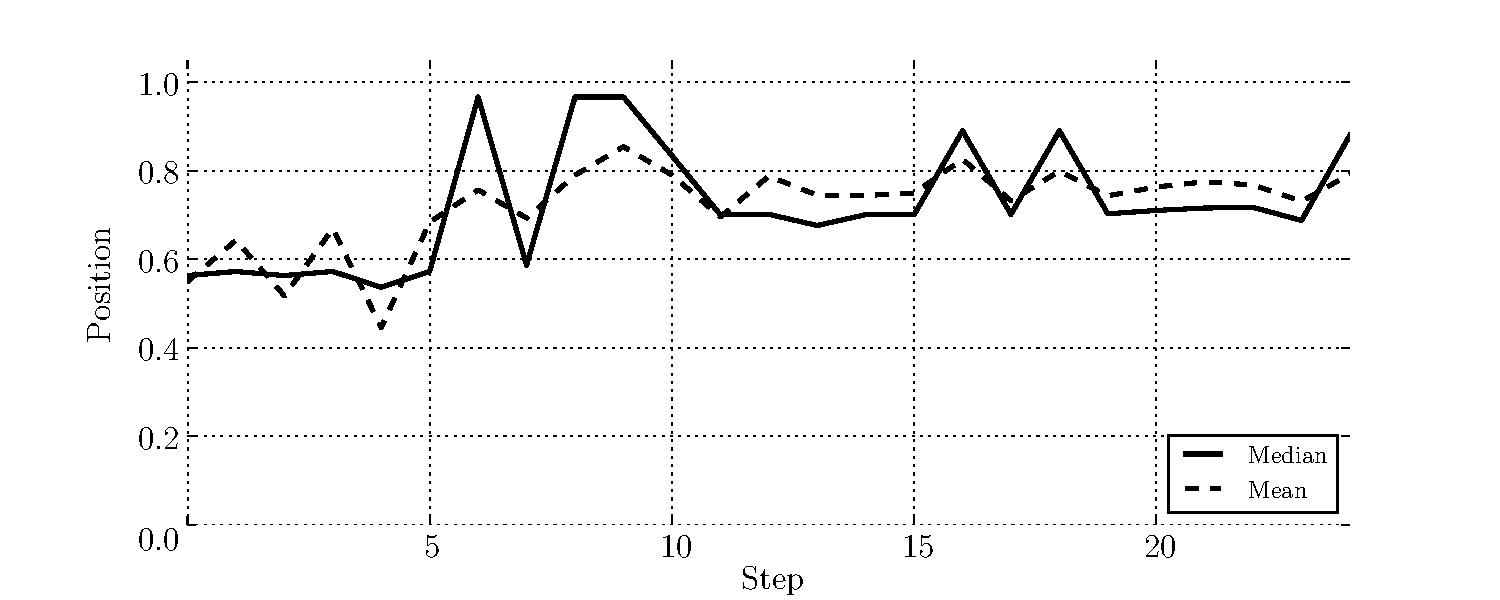
\includegraphics[width=\textwidth]{ColdWar/Figures/Exp4_uswin_trace}
        \caption{Experiment 4}
    \end{subfigure}

    \caption{Example Model Traces -- Median Positions}
    \label{fig:example_traces}
    \figSpace
\end{figure}

\begin{figure}[!htbp]
    \centering
    \begin{subfigure}[t]{0.75\textwidth}
        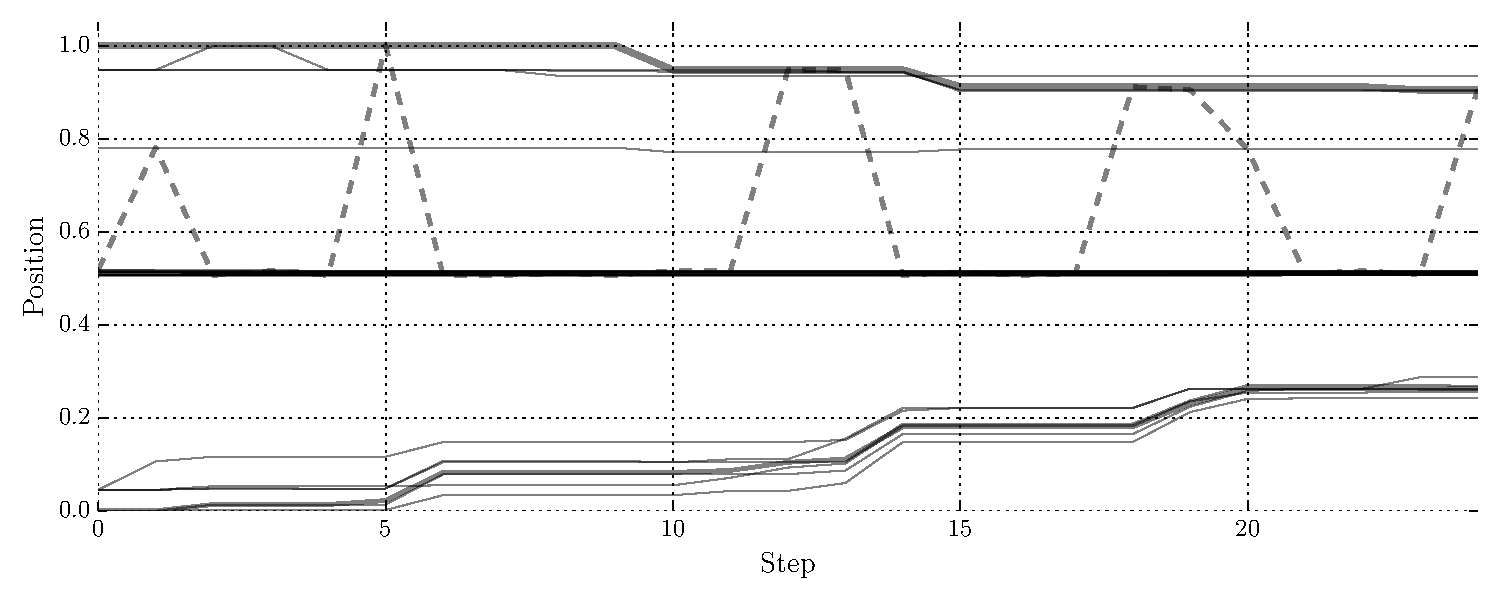
\includegraphics[width=\textwidth]{ColdWar/Figures/Exp1_agent_traces}
        \caption{Experiment 1}
    \end{subfigure}

    \begin{subfigure}[t]{0.75\textwidth}
        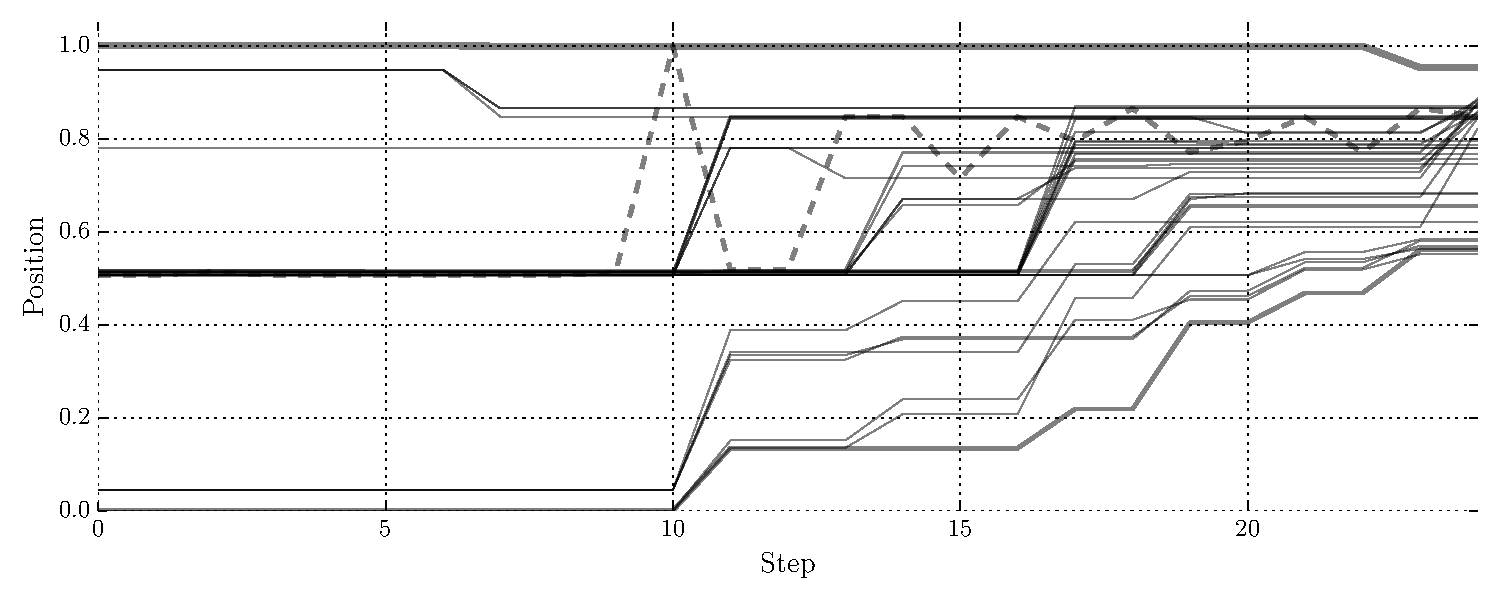
\includegraphics[width=\textwidth]{ColdWar/Figures/Exp2_agent_traces}
        \caption{Experiment 2}
    \end{subfigure}

    \begin{subfigure}[t]{0.75\textwidth}
        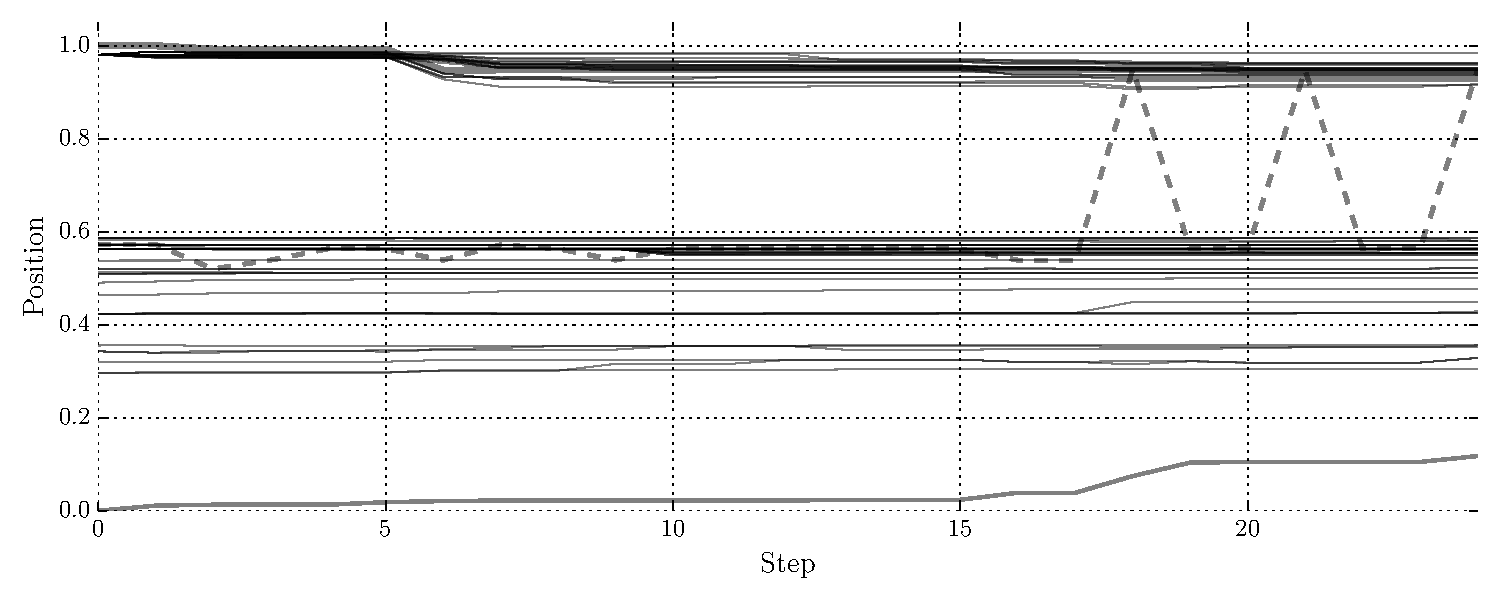
\includegraphics[width=\textwidth]{ColdWar/Figures/Exp3_agent_traces}
        \caption{Experiment 3}
    \end{subfigure}

    \begin{subfigure}[t]{0.75\textwidth}
        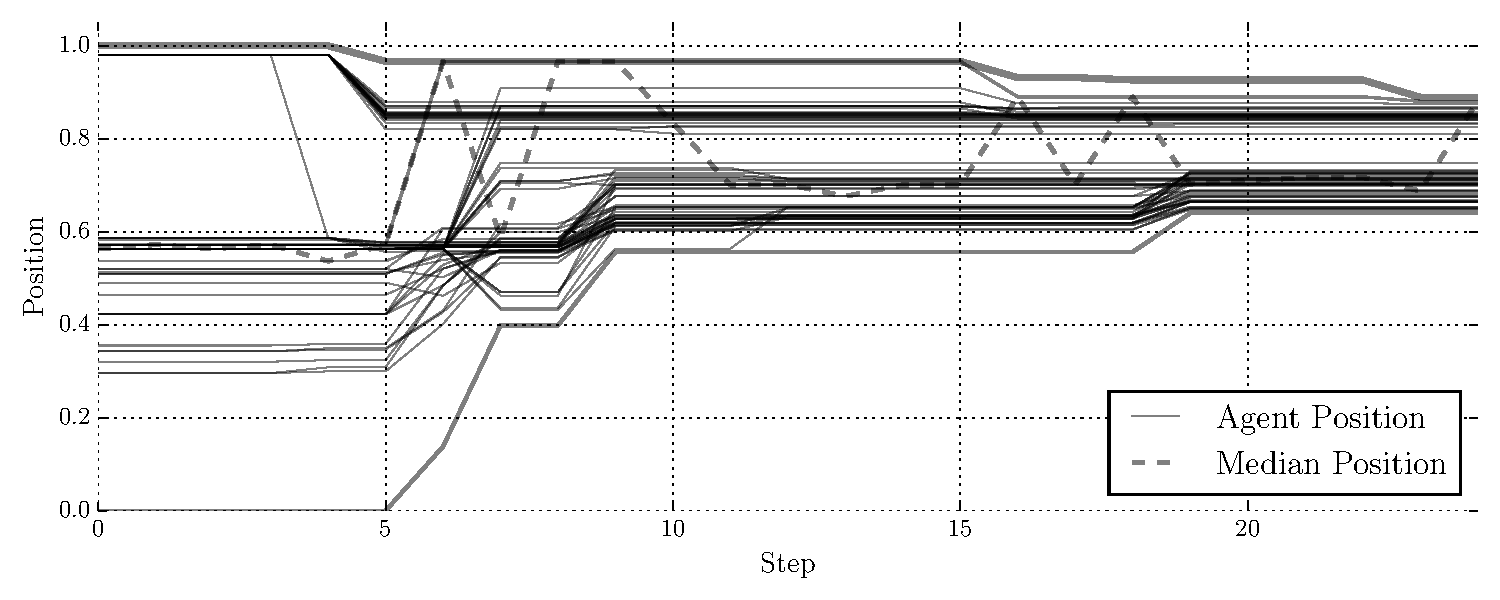
\includegraphics[width=\textwidth]{ColdWar/Figures/Exp4_agent_traces}
        \caption{Experiment 4}
    \end{subfigure}

    \caption{Example Model Traces -- Agent Positions}
    \label{fig:example_agent_traces}
    \figSpace
\end{figure}

\subsection{Predicted Conflicts}

The models do not only generate overall positional traces, but simulated events, and conflicts in particular. These conflicts are an important part of the simulated history, not only because they can drive substantial changes in agent positions but because they provide useful anchor-points for comparing model runs to real history. We have robust historic data on wars and lesser militarized interstate disputes, and a well-developed understanding of international partnerships and rivalries, which allow us to assess the plausibility of the conflicts the model produces. Furthermore, conflicts are an important area for prediction and forecasting, and it is valuable to assess whether these models can be used for such prediction.

Each model run in each experiment collects the conflict events generated across all run steps; for each, the code computes the mean number of conflicts occurring between each dyad of agents across all models. These dyads are undirected, since in the model variants applied here both parties must mutually decide to start a conflict for it to occur. These simulated conflict counts are then merged with the count of militarized interstate disputes for each dyad, as described above.

The correlations between the predicted and observed number of conflicts are small. Most conflicts generated by the model do not reflect real conflicts, while most real conflicts are not mirrored in the simulated data. Nevertheless, we may still ask whether the model provides any statistically useful information. In order to do so, I run two regressions on each experiment output, with predicted conflicts as the independent variable: a linear regression, with observed MIDs as the dependent variable, shown in Table \ref{table:mids_linear}; and a logistic regression, with a dependent dummy variable for the presence of any MIDs on the dyad, in Table \ref{table:mid_logits}. The model generates relatively few conflicts -- like real-world wars, these are rare events \citep{king_2001}, meaning that the mean conflicts values are small, leading to large-magnitude coefficients. 

First, let us examine the linear regressions. Note that we have no particular reason to believe that the relationship between the number of model-generated and observed conflicts is linear. However, if more simulated conflicts do in fact predict more observed conflicts, we would expect the coefficient to be positive. In fact, all the coefficients are positive, and all but the one for Experiment 1 are statistically significant, suggesting that the models are generating some useful information as to the number of observed conflicts.

Further evidence of this is visible in Table \ref{table:mid_logits}. These regressions test whether more model conflicts between dyads of actors predict \emph{any} conflicts occurring in the relevant time period. In this case the coefficient values are positive and significant across all the models, indicating that when the model predicts more conflicts between a pair of countries, we are indeed more likely to have observed at least one conflict between them in the historic data.

While $R^2$ is an imperfect measure of the goodness-of-fit of a statistical model, it is an acceptable way of comparing models of the same type and the same dependent variable \citep{wooldridge_2008}. The $R^2$ values across all models are low, indicating that they are explaining only a small fraction of the variance observed in the MID data. Nevertheless, we can see that the $R^2$ value on the Experiment 4 linear regression is an order of magnitude better than for the other experiments, and that this is not the case for the logistic regression. This suggests that the model is more accurately predicting the number of conflicts, conditional on conflicts occurring at all. Across both types of regressions, furthermore, we can see that Experiment 3 has the least explanatory power.


\begin{table}
  \begin{center}
  \caption{Militarized Interstate Disputes -- Linear Regressions}
  \label{table:mids_linear}
  \begin{tabular}{lcccc}

  \hline
                      & Experiment 1 & Experiment 2 & Experiment 3 & Experiment 4  \\
  \hline
  Const.               & 1.043***     & 1.014***     & 0.392***     & 0.362***      \\
                       & (0.183)      & (0.173)      & (0.049)      & (0.044)       \\
  Model Conflicts      & 1.473        & 8.327***     & 17.409***    & 1015.746***    \\
                       & (1.235)      & (1.950)      & (5.090)      & (40.768)     \\
  \hline
  Adjusted $R^2$     &     0.001      &   0.027      &  0.004       &   0.195 \\            
  \hline
  \hline
  \multicolumn{4}{l}{Standard errors in parentheses.} \\
  \multicolumn{4}{l}{* $p<.1$, ** $p<.05$, *** $p<.01$} \\
  \end{tabular}
  \end{center}
  \tableSpace
\end{table}

\begin{table}
  \begin{center}
  \caption{Militarized Interstate Disputes -- Logistic Regressions}
  \label{table:mid_logits}
  \begin{tabular}{lcccc}
  \hline
                      & Experiment 1 & Experiment 2 & Experiment 3 & Experiment 4  \\
  \hline
  Const.               & -1.300***    & -1.422***    & -2.201***    & -2.197***     \\
                       & (0.101)      & (0.111)      & (0.067)      & (0.066)       \\
  Model Conflicts & 1.952***     & 27.658***    & 19.739***    & 654.501***    \\
                       & (0.622)      & (7.190)      & (4.556)      & (148.758)     \\
  \hline
  McFadden's $R^2$     &  0.015       &  0.030       & 0.009        & 0.016 \\
  \hline
  \hline
  \multicolumn{4}{l}{Standard errors in parentheses.} \\
  \multicolumn{4}{l}{* $p<.1$, ** $p<.05$, *** $p<.01$} \\
  \end{tabular}
  \end{center}
  \tableSpace
\end{table}

It is also useful to look at the specific conflicts being predicted. Table \ref{table:conf_dyads} shows the top ten most frequently predicted conflict dyads for each experiment. One finding that stands out here is that the Baseline and Updated models appear to generate two different classes of conflcit. The Baseline model generates no direct conflicts between the two rival superpowers in either Experiment 1 or 3, and very few even directly involving either. Instead, the conflicts are largely between lower-tier agents, with positions closer to the median. In historic terms, these are proxy wars: the belligerents are not the superpowers themselves, but each draws some support from a different superpower and its close allies. These contributions are often small, as their preference for one side over the other may be relatively weak. The stakes of the conflicts, in terms of the overall orientation of the simulated international system, are correspondingly weak. In contrast, the Updated model sees much more direct involvement by the two main superpowers directly, including direct conflicts between them. The conflicts that are not between the two superpowers directly appear to often take the form of one superpower (most often the USA) attempting to coerce a much weaker country.

%Belgium is especially over-represented in the conflicts generated in both Experiments 1 and 3. This appears to be driven by its combination of relative strength and location close to the median (in Experiment 1, its own position is frequently the median position), making it a particularly influential actor in the simulated international system. In contrast, the Updated model generates many conflicts involving the USA and USSR agents, including frequent direct conflicts between the two.

\begin{table}
  \begin{center}
  \caption{Top Predicted Conflict Dyads}
  \label{table:conf_dyads}
  \begin{tabular}{l|l}
  \hline
  Experiment 1 & Experiment 2 \\
  \hline
  \begin{tabular}{ll}
  England & Iraq \\
  Egypt & England \\
  Belgium & France \\
  Belgium & Iran \\
  Argentina & USA \\
  Belgium & Egypt \\
  Argentina & Brazil \\
  Egypt & Iraq \\
  Belgium & Netherlands \\
  Argentina & Canada
  \end{tabular} & \begin{tabular}{ll}
    Bulgaria & USA \\ 
    USSR & USA \\ 
    USA & Yugoslavia \\ 
    China & USA \\ 
    England & USSR \\ 
    Australia & USA \\ 
    China & England \\ 
    Poland & USA \\ 
    Bulgaria & England \\ 
    Czechoslovakia & USA 
  \end{tabular} \\
  \hline
  Experiment 3 & Experiment 4 \\
  \hline
  \begin{tabular}{ll}
    Egypt & Jordan \\
    France & Turkey \\
    Belgium & Netherlands \\
    France & Iran \\
    Belgium & Bulgaria \\
    Afghanistan & Saudi Arabia \\
    Belgium & Luxembourg \\
    Czechoslovakia & Romania \\
    Poland & Hungary \\
    Turkey & Iran
  \end{tabular} & \begin{tabular}{ll}
    USA & USSR \\ 
    USA & United Kingdom \\ 
    USSR & Argentina \\ 
    USA & India \\ 
    USA & Yugoslavia \\ 
    USA & China \\ 
    USA & Czechoslovakia \\ 
    China & France \\ 
    USA & Portugal \\ 
    USA & Poland
  \end{tabular} \\
  \hline
  \end{tabular}
  \end{center}
  \tableSpace
\end{table}

% WGK: 8. Is there a missing dyad for experiment 4 in Table 2.7?  Why the blank line? Were there only 9 dyads? 
% --> There are 10 there, the line spacing format is just weird

Several of the predicted conflict dyads stand out as being particularly plausible, or implausible. The United States and Soviet Union, with high conflict counts in Experiments 2 and 4, are the most frequent dyad observed in the MID dataset for the 1948-98 period. However, these disputes never escalated to a full military conflict. Such a conflict, if it had occurred, would likely have had catastrophic consequences far outside the scope of this model. Interestingly, despite not incorporating geography, the Baseline model generates several regional conflict dyads which are in fact observed in reality, including Egypt and Iraq \citep{podeh_1995} and Brazil-Argentina \citep{mariano_2013} -- though, again, these real-world rivalries were of relatively low military intensity.

Some of the implausible conflicts may be artifacts of the model input data. For example, the conflicts between the United States and the United Kingdom (UK) are attributable to the UK's initial position, which in both the Original and Updated data is close to 0.5. However, this is almost certainly an underestimate of its alignment with the United States, particularly in light of the signing of the North Atlantic Treaty \citep{treaty_1949} in the following year. Similarly, far from being in conflict with one another, Belgium, France, and the Netherlands were all parties to the Treaty of Brussels of 1948, which included a mutual defense guarantee \citep{treaty_1948}. This highlights the degree to which the year chosen to use to instantiate the model can influence the results, as well as the information missing from the tau-b similarity measurement. Furthermore, as mentioned previously, several countries which would be pivotal to the Cold War, such as Vietnam, and West and East Germany, were not yet sovereign in 1948, and are excluded from the input data -- making it impossible to generate any conflicts involving them.
%% WGK: Write more here to describe proxy wars, etc. DONE

\subsection{Predicted Alliances}

In addition to conflicts, the other detailed output the model produces is the position of each agent at each step. The space in which these positions exist is fairly abstract, particularly in this example. While in some cases positions can be assigned concrete meaning on a particular issue (e.g. number of years before a policy is adopted, as in \citet{stokman_1994b}), in this case, the positions simply indicate alignment with the security interests of the United States or Soviet Union, as anchored in the starting year. The specific issues underlying these interests, however, obviously change substantially over the course of the time period we are concerned with, and assessing the position of each country across such issues is a substantial and ill-defined task in and of itself. Furthermore, both superpowers can and occasionally do change their own position as well, suggesting that they are compromising some interests in order to maximize their security with regard to the current state of the world.

One way around needing to interpret the position space is to examine not the specific positions themselves, but the distance between the positions held by two agents. Within the model, when agents' positions are closer, they are more likely to assist each other more strongly in conflicts. Furthermore, this fact is public -- all other agents know it, and explicitly take it into account when estimating the probabilities of winning or losing potential conflicts. This behavior bears a clear resemblance to alliances, an enduring institution in international relations (both in practice and theory). Indeed, the Realist school of thought often holds that alliances and treaties are not meaningful in and of themselves, but only inasmuch as they reflect an underlying alignment of states' interests \citep{walt_1987}. With this in mind, I hypothesize that if a model is capturing aspects of real state behavior, the closer two agents are, the more likely the relevant countries are to have some sort of alliance or other formal defense or security agreement.

In order to test this hypothesis, I use the Correlates of War \citep{gibler_2009,gibler_2013} alliance data. Recall that this dataset served to generate the model inputs as well; The variable I attempt to predict is alliances in effect in 1998 (corresponding approximately to end-year of the number of steps the model has run for), reducing the risk of circular prediction. Furthermore, for experiments 1 and 2, I am using the Original Input data, while the 1998 alliances are drawn from the most recent COW data; as noted in Section \ref{sec:input_data}, there appears to be substantial enough difference between the older and updated datasets to further reduce the risk of circular prediction.

I compute the distance between the positions of each pair of agents at the end of each run, and then find the average of these distances across each experiment. I then merge the resulting data from each experiment with the dyadic alliance data, padded to include 0 values for each pair of states for which no agreement is recorded. With these merged datasets, I run two models: a multinomial logistic regression \citep{mcfadden_1984}, and an exponential random graph model \citep{robins_2007}. 

% 9. On page 60, the page after table 2.8, there is a reference to exponential random graph models. I suggest this needs a citation.


\begin{table}
  \begin{center}   
    \caption{Alliance Type -- Multinomial Choice Logistic Regression}
    \label{table:mc_logit_results}
  \begin{tabular}{lcccc}
  \hline
                & Experiment 1 & Experiment 2 & Experiment 3 & Experiment 4 \\
  \hline
  \multicolumn{5}{l}{Alliance=1}                                            \\
  \hline
  Const         & -6.828***    & -8.060**     & -7.387***    & -8.484***    \\
                & (1.917)      & (2.429)      & (1.601)      & (1.459)      \\
  Mean Distance & 2.540        & 9.158        & 2.586        & 50.793**     \\
                & (4.019)      & (7.667)      & (3.559)      & (20.673)     \\
  \hline
  \multicolumn{5}{l}{Alliance=2}                                            \\
  \hline
  Const         & -4.902***    & -5.003***    & -5.660***    & -5.211***    \\
                & (0.863)      & (1.327)      & (0.897)      & (1.270)      \\
  Mean Distance & 0.044        & 0.624        & -1.554       & -37.990      \\
                & (2.472)      & (6.523)      & (2.921)      & (56.118)     \\
  \hline
  \multicolumn{5}{l}{Alliance=3}                                            \\
  \hline
  Const         & -4.043***    & -4.332***    & -4.073***    & -3.915       \\
                & (0.544)      & (0.763)      & (0.417)      & (0.607)      \\
  Mean Distance & 0.893        & 2.843        & -2.087       & -29.748      \\
                & (1.393)      & (3.386)      & (1.439)      & (25.521)     \\
  \hline
  \multicolumn{5}{l}{Alliance=4}                                            \\
  \hline
  Const         & -0.974***    & -0.056       & -0.080       & -1.2184***   \\
                & (0.150)      & (0.329)      & (0.086)      & (0.122)      \\
  Mean Distance & -3.286***    & -9.905***    & -7.792***    & -5.716       \\
                & (0.660)      & (2.231)      & (0.529)      & (4.214)      \\
  \hline
  \hline
  \multicolumn{5}{l}{Standard errors in parentheses.} \\
  \multicolumn{5}{l}{* $p<.1$, ** $p<.05$, *** $p<.01$} \\
  \end{tabular}
  \end{center}
  \tableSpace
\end{table}

The logistic regression treats each dyad as independent, and attempts to predict which category the relationship between the two states falls into. Across all four experiment results, shown in Table \ref{table:mc_logit_results} the mean distance between agents is not a significant predictor of ententes, non-aggression or neutrality agreements (alliance categories $1-3$, as detailed in Table \ref{table:alliance_types}). However, in Experiments $1-3$, for defense pacts (category 4, the strongest type of relationship), the model mean distance is statistically significant, with a negative sign. This means that the smaller the distance between the agents (which is to say, the closer they are), the more likely an alliance becomes. This is not the case with Experiment 4. Though the coefficient is still negative, it is not significant.

A key assumption of a logistic regression is that the observations are independent. However, we know that this is not the case with regard to interstate relationships in general, and alliances in particular. Rather, the alliances form a network, and should be studied as such \citep{maoz_2010}. In order to test whether the model distances are a useful predictor of the alliance network, I use exponential random graph models (ERGMs), a methodology developed specifically to account for such networked interdependence. The independent variable here is the simplified alliance network, where the nodes are states, connected by an edge wherever a defense pact ($Alliance=4$) relationship exists. The key independent variable is the generated Mean Distance values, as with the logistic regression. Following \citet{cranmer_2012b}, I include a \emph{2-star} coefficient (the number of pairs of edges, or trios of connected nodes) in order to capture the structural effect whereby states with more allies tend to attract additional allies (which \citet{cranmer_2012b} term the `popularity effect'). 

\begin{table} 
  \centering 
    \caption{Alliance Network -- Exponential Random Graph Models} 
    \label{table:ergm_results}  
  \begin{tabular}{@{\extracolsep{5pt}}lcccc} 
  \\[-1.8ex]\hline 
  \\[-1.8ex] & Experiment 1 & Experiment 2 & Experiment 3 & Experiment 4\\ 
  \hline \\[-1.8ex] 
   2-star & $-$0.188$^{***}$ & $-$0.171$^{***}$ & $-$0.023$^{***}$ & $-$0.031$^{***}$ \\ 
    & (0.017) & (0.017) & (0.003) & (0.003) \\ 
    & & & & \\ 
   Mean Distance & $-$2.113$^{***}$ & $-$5.613$^{***}$  & $-$6.308$^{***}$ &  $-$25.981$^{***}$ \\
                 & (0.607)         &    (1.245)        &   (0.615)         &      (4.589)     \\ 
  \hline 
  \hline
  \multicolumn{5}{l}{Standard errors in parentheses.} \\
  \multicolumn{5}{l}{* $p<.1$, ** $p<.05$, *** $p<.01$} \\
  \end{tabular}
  \tableSpace
\end{table} 

The results of this model are shown in Table \ref{table:ergm_results}. The key finding here is that the Mean Distance between actors is still a significant, and negative, predictor of an alliance between them, even when taking the network structure into account. Note that unlike with the logistic regression, here Experiment 4 Mean Distances are significant as well.

\section{Discussion} \label{cw_discussion}

% [WGK:] 3. The end of the chapter also does not provide a road sign on what progress is made on the dissertation by this chapter. I suggest both are needed.


%This chapter set out to accomplish several goals: to attempt to reproduce the results of \citet{bdm_1998}; to test the Expected Utility Model more rigorously, by examining it not only qualitatively but by using its outputs as predictors of real data; and to compare several model variants against one another, to see where they differ, how, and why, and to test which has the most explanatory or predictive power.

This chapter set out to accomplish several goals. The first was to attempt to reproduce the results of \citet{bdm_1998}, in order to test my reimplementation of the Expected Utility Model's power to explain and predict the long-term course of complex international competition. It also extended the analysis presented in the original paper by collecting additional model outputs and quantitatively testing their correspondence with empirical data. Additionally, this chapter continued to comparatively test the EUM variants presented in Chapter 2, by implementing the Baseline model against the variant with the highest explanatory power on the ICEWS dataset; if the theories embedded in the model variant are in fact more explanatory of the world than the Baseline's, we would expect that variant to have more explanatory power here as well. If it does not, that would indicate either that the results of the previous chapter are due to chance, or that the dynamics driving international relations during the Cold War are different than those driving them in the 2004-06 timeframe that we previously examined.

I was unable to reproduce the model inputs from contemporary data. This highlights two issues. One is the quality of the input data: the alliance network which I used is an updated version of the one used to generate the Original Input data, and as such is intended to be more accurate \citep{gibler_2013}. In order to use the methodology presented here for forecasting, we must explicitly be aware that input data sources may be incomplete or contain errors, and if possible account for that possibility explicitly (e.g. by performing sensitivity analyses on the input data). The other issue is the need for explicit clarification of the pre-processing steps needed to get from the raw input data (in this case, the alliance network) to the actual model input (in particular, the agent positions). As shown in Section \ref{sec:input_data}, the method described for generating agent positions in fact produces a two-dimensional position space; the paper does not specify the heuristic or projection used to reduce this space to one dimension.

Despite being unable to reproduce the Original Inputs from raw data, I was able to instantiate my model runs using the input data provided in the original paper. The overall distribution of outcomes produced by my reproduction of the original model is qualitatively similar to the output described in the original paper, though not identical. The original paper appears to generate a wider range of outcomes, and in particular more USSR-leaning ones than the reproduction model. Furthermore, the individual run traces do not appear to be a good match to the examples presented in the original paper. While the stochastic nature of the model makes it essentially impossible to reproduce specific model traces without access to the original source code and random seed, the example traces reported in the original appear to show more movement of individual agent positions than characterize my reproduction, while the median position does not have the saw-tooth pattern which characterizes all the experiments, but in particular Experiments 1 and 3. 
Experiment 3, using the Updated Input data, generates similar behavior by the median and individual agent positions to Experiment 1. This suggests that the lack of major, stable shifts in the median position is a feature of this particular model variant, rather than the particular input configuration of agents, positions, and capabilities. Recall that as demonstrated in the deep dive in the previous chapter (Section 3.3.2), cascades of agents backing out of offers in response to other agents accepting their own offers leads to an overall reduction in agent movement.

As I discussed above and in the previous chapter, a close examination of my reproduction model suggests that the stability of the median across its runs is driven by the rule allowing agents to renege on an accepted offer if another agent has accepted their own offer. This rule is part of the offer selection sub-model, which is one of the least-specified sub-models not only in \citet{bdm_1998} itself but in the other descriptions of the model as well. There are two possibilities: one is that, despite my best efforts, I have not implemented this model behavior to match the description. The second is that the descriptions of this behavior in the prior material do not accurately reflect the behavior of original the underlying source code. As the original code is not available to inspect, it is impossible to verify directly which possibility is correct. 

Nevertheless, there is at least anecdotal evidence that the flaw is not in my replication but in the original description. Private communications with scholars familiar with the original paper have suggested that the experiments it describes were implemented using the commercial version of the model software, developed by Bueno de Mesquita's consulting firm, Decision Insights, Incorporated (DII). This software was the subject of litigation, during which Gary Slack, a DII employee who is thanked for ``invaluable programming assistance'' in \citet{bdm_1998}, testified that the model contains proprietary methods not disclosed in the public literature \citep{dii_2011}. This suggests, in turn, that the model description in the original paper, and the prior literature more broadly, is incorrect or incomplete. In this case, the difference between the described and observed model appears to be attributable to a specific sub-model -- how agents select offers and change position. I believe that sub-model is indeed a key place where the public and proprietary versions of the model diverge. In fact, the traces in Experiment 2, where agents cannot back out of selected offers, appear to be qualitatively more similar to the traces reported in the original paper than Experiment 1.

While replication is certainly important, a more interesting question is how well the models reproduce the observed history of the Cold War and its end. Historically, while the end of the Cold War was sudden and unexpected, it was not a short-lived phenomenon, at least on the time-scale we are modeling here. In fact, it was followed by a decade or more of `unipolarity' during which many countries formerly oriented towards the USSR, and often allied with it, rapidly shifted their international position towards the United States and its allies \citep{wohlforth_1999}. The most notable demonstration of the long-term transition in the international geopolitical orientation is was the countries who were formerly members of the Soviet-led Warsaw Pact alliance joining NATO, the US-led alliance which had been the Warsaw Pact's primary adversary \citep{waltz_2000}. While there is only one run of history for us to examine, it is worth noting that Cold War-era fiction envisioning Soviet ascendancy \citep[e.g.][]{milius_1984} described a similar process happening in reverse, with NATO countries being rapidly pulled into the USSR's orbit. Examination of the example model traces shown in Figure \ref{fig:example_agent_traces}, and other traces not shown here, indicate that the replication model of Experiments 1 and 3 does not tend to produce such sharp, stable transitions. In contrast, Experiments 2 and 4 do feature relatively sharp changes, with Soviet-aligned agents moving towards the United States followed by the Soviet Union itself. Qualitatively, at least, these models appear to be generating behaviors which mirror the historic record. Note, however, that the majority of model runs across all experiments do not follow this behavior, and indeed do not generate a `victory' to one superpower or the other.

None of the experiments presented here appear to be be powerful predictors of observed conflicts. While the coefficients are statistically significant, they are nevertheless only weak predictors of observed militarized disputes in the relevant historic period. There are several possible explanations here. One is that model conflicts do not play the same role as do MIDs in the international system, at least at the scale and with the issues being examined here. The model's single dimension means it is most likely to generate conflicts driven by the overall `issue' -- in this case, the competition between the two superpowers. However, many conflicts arise due to issues particular to a state, dyad or region \citep{senese_1996}. If these issues are not embedded in the initial position-generating alliance network, the model will obviously be unable to account for them, and thus will not generate conflicts driven by them. Furthermore, the model lacks a spatial component. Many conflicts are between neighbors, and may be driven at least in part by disputes arising due to that relationship -- with territory being the most obvious example, though not the only one. The ability of other states to assist one side or another in a conflict is also influenced by geography: in terms of sending military forces or assistance, but also in terms of `softer' power. For example, nearby states trade more than far-away ones \citep{ramanarayanan_2011}, meaning that overall, a state's ability to affect another by increasing or decreasing trade and commerce is also tied to the distance between them. Finally, by only examining militarized disputes, we may be missing other forms that conflicts take, and that states use to coerce one another, such as via diplomatic or economic means.

Similarly, the models are significant but not powerful predictors of alliances. They appear most capable of predicting defensive alliances, the strongest category: the closer the final positions of two agents are, the more likely they are to have a defensive pact between them, committing one to come to the other's aid if attacked. Of the alliance types coded in the COW data, defensive pacts most closely mirror the behavior coded in the model itself, with agents more likely to contribute more resources to a closer agent when that agent is involved in a conflict. This correspondence suggest that the model is indeed capturing one dimension of states' decisionmaking. Importantly, the dyad-wise position distances are a stronger predictor in the Experiments 2 and 4, where the agents tend to change positions more than in Experiments 1 and 3. This indicates that the dynamics of the models are generating useful information not directly present in the initial data.

We have already touched on comparing the experiments to one another in the various sections above. A common thread is that the Updated model outperforms the Baseline model: The agent behaviors it generates are more qualitatively plausible, and the conflicts it generates are more predictive of real conflicts across both input sets. Note that the one exception is the prediction of alliances in Experiment 4. Though this experiment generates the best predictions of conflicts, it also produces the worst predictions of alliances. It is somewhat surprising that these two metrics do not go together, since we would hope that the most accurate model of the system would generate strong predictions for both. One possible explanation is suggested by the fact that Experiment 4 generates the fewest outcomes with one side or another gaining a decisive advantage. Nearly all of its outcomes involve the Cold War continuing indefinitely, and (as Figure \ref{fig:model_traces} shows) becoming more stable. In contrast, the target alliance network is from 1998, reflecting a decisively post-Cold War world. Thus, the experiment may be predicting conflicts likely to occur in a Cold War context, which accounts for the bulk of the time (and the conflicts) being studied; however, since it does not predict an end to the Cold War, it fails to predict the alliance network which follows. 

This analysis provides more evidence for the value of comparatively applying multiple models. The better fit of the Updated model is consistent with the results of Chapter 3, giving us confidence that, across different input datasets capturing different historic periods at different scales, the assumptions of the Updated EUM variant -- particularly agents not changing position due to conflicts, and not reneging on accepted offers -- provide better models of actual state behaviors. Furthermore, this chapter demonstrates another form of comparative modeling: the use of different input datasets which all attempt to capture the same underlying state of the world. In this case, these are the two input sets, derived from different versions of the Correlates of War capabilities and alliance data. Using these, we can see the qualitatively different behavior in particular between Experiments 2 and 4, where the same Updated model is instantiated with the two different input datasets. There does not appear to be a simple, reduced explanation for this difference. Rather, the particular configurations of the two inputs yield substantially different distributions of outcomes, highlighting the uncertainty present in the model itself.

Finally, let us pull back to examine the original question which motivated \citet{bdm_1998}: whether the end of the Cold War could be explained by contemporary theories of international relations, as operationalized by the Expected Utility Model. The answer here appears to be a qualified `yes'. Despite the differences in the behavior and dynamics of the different model variants and input data, all experiments generate an overall prediction of an advantage to the United States, despite the initial balance of power being nearly completely even. This suggests that the initial hypothesis is correct, and that the end of the Cold War was potentially predictable from much earlier data. In fact, this analysis provides more evidence for the robustness of the US advantage, as it recurs across several model variants, indicating it is not simply an artifact of one particular model implementation. Nevertheless, the end of the Cold War is far from inevitable, even within these models; if these models are capturing some of the true underlying dynamics, the results suggest that the end of the Cold War was surprising not solely because it was emergent, but because it was in fact an unlikely event. Furthermore, these results show the caution we must exercise in using such model for prediction. While the input data may have been knowable in the starting year, we necessarily used knowledge from future years to assess the model outputs, and determine that the conflicts were non-predictive while the positions were. More research is required to assess whether these are general features of the model, or outcomes specific to this particular case or system scale.